% \section{Silná a slabá formulace 1D okrajové úlohy 2. řádu}
% 
% Řešme jednoduchou úlohu vedení tepla. 
% 
% Představme si zjednodušeně termosku jako 1D úsečku (oblast $\Omega = [0,1]$),
% která na jedné straně (na dně) nepropouští žádné teplo a na straně druhé je otevřená,
% tedy v kontaktu s okolím o referenční teplotě 0 (řekněme, že tu můžeme libovolně škálovat, např. že odpovídá 25$^\circ$C).
% 
% Zaveďme si veličinu $q(x,t)$, která bude popisovat hustotu energie (tepla) uvnitř oblasti $\Omega$.
% Oblast $\Omega$ je interval, jedná se tedy v tomto případě o délkovou hustotu.
% Může se samozřejmě měnit v čase $t$.
% Celkovou energii v oblasti $\Omega$ v čase $t$ tedy vyjádříme jako
% \[
%   \int\limits_0^1 q(x,t) \d x
% \]
% Dále si zaveďme tepelný tok $j(x,t)$, který vyjadřuje kolik energie projde bodem $x$ (představujeme si příčný průřez termoskou)
% za jednotku času.
% Nyní můžeme vyjádřit úbytek energie jako zápornou změnu celkové energie v čase a tu položit rovnu rozdílu tepelného toku
% na začátku a konci oblasti, tedy v bodech $x=0$ a $x=1$.
% \[
%   -\frac{\partial}{\partial t}\int\limits_0^1 q \d x = j(1) - j(0) = \int\limits_0^1 \frac{\partial j}{\partial x} \d x
% \]
% Dostali jsme energetickou bilační rovnici. Pokud budeme předpokládat, že $j$ je hladkou funkcí podle $x$, můžeme rozdíl tepelných toků nahradit 
% integrálem derivace $j$ přes danou oblast.
% 
% Dále si můžeme představit, že stěny termosky přece jen nejsou ideální a i přes ně probíhá výměna tepla.
% Tedy zavedeme funkci $f(x)$, která bude popisovat dodávání ($f(x)>0$) nebo odebírání ($f(x)<0$) energie z venku do/z oblasti $\Omega$.
% Tím získáme následující bilanční rovnici:
% \[
%   -\frac{\partial}{\partial t}\int\limits_0^1 q \d x = j(1) - j(0) + \int\limits_0^1 f(x) \d x= \int\limits_0^1 \left(\frac{\partial j}{\partial x} + f(x) \right) \d x
% \]
% 
% ....
% 
% \[
%   \frac{\partial q}{\partial t} + \frac{\partial j}{\partial x} = f(x)
% \]
% Pokud budeme uvažovat ustálenou úlohu, tedy časově neměnnou, zjednoduší se rovnice na
% \begin{equation}
%   j'(x) = f(x) \label{eqn:continuity_steady_1d}
% \end{equation}
% 
% Nyní připomeňme Fourierův zákon, který definuje tepelný tok pomocí gradientu teploty
% \begin{equation}
% j(x) = -K(x)u'(x), \label{eqn:fourier_1d}
% \end{equation}
% kde $K(x)$ je tepelná vodivost materiálu.
% 
% 
% Pokud nyní dosadíme \eqref{eqn:fourier_1d} do \eqref{eqn:continuity_steady_1d}, dostaneme Poissonovu rovnici,
% a poté popíšeme náš problém termosky
% % \[
% % -(K(x)u'(x))' = f(x)
% % \]
% 
% \begin{eqnarray}
% -(Ku')'(x) &=& f(x) \qquad \textrm{in } \Omega = [0,1], \label{eqn:poisson}\\
% -(Ku')(0) &=& 0, \label{eqn:hom_neumann}\\
% u(1) &=& 0, \label{eqn:hom_dirichlet}
% \end{eqnarray}
% kde \eqref{eqn:poisson} řídí rozložení teploty $u(x)$ uvnitř termosky,
% \eqref{eqn:hom_neumann} je homogenní Neumannovou okrajovou podmínkou a vyjadřuje nulový tepelný tok skrz dno termosky
% a \eqref{eqn:hom_dirichlet} je homogenní Dirichletovou okrajovou podmínkou a pokládá teplotu na otevřeném konci termosky rovnou nule.
% 
% 
% Slabou formulaci získáme přenásobením \eqref{eqn:poisson} testovací funkcí $\varphi(x)\in\mathcal{C}([0,1])$, $\varphi(1)=0$, 
% následnou integrací rovnice přes oblast $\Omega$ a aplikací okrajových podmínek za použití per partes (resp. Greenovy věty).
% \[
%   \int\limits_{\Omega} -\left( Ku'\right)'(x) \varphi(x) \d x = \int\limits_{\Omega} f(x) \varphi(x) \d x
% \]
% 
% \begin{equation}
% \left[-\left( Ku'\right)(x)\varphi(x)\right]_0^1 + \int\limits_0^1 \left( Ku'\right)'(x) \varphi'(x) \d x
%     = \int\limits_0^1 f(x) \varphi(x) \d x\label{eqn:weak_form}
% \end{equation}
% První člen daný okrajovými podmínkami je v našem případě nulový, díky Neumannově okrajové podmínce a volbě $\varphi$.
% 
% Integrální rovnici \eqref{eqn:weak_form} nazýváme slabou formulací problému \eqref{eqn:poisson}-\eqref{eqn:hom_dirichlet}.
% Všimněme si dvou vlastností této formulace:
% \begin{itemize}
%   \item $u''$ nemusí existovat
%   \item $u'$ nemusí být spojitá, stačí existence integrálu $\int_0^1(u')^2 \d x$
% \end{itemize}
% 
% Označme nyní prostor, ze kterého pochází funkce $\varphi$:
% \begin{equation}
%   V = \{v\in H^1(\Omega); v(0) = 0\},
% \end{equation}
% kde prostor $H^1(\Omega)$ zaručuje pro funkce $\varphi$ výše zmíněnou druhou vlastnost,
% a kde dále vidíme závislost $V$ na Dirichletově okrajové podmínce.
% Z tohoto prostoru bude pocházet i řešení $u\in V$.
% 
% \paragraph{Galerkinova aproximace}
% Nyní zvolíme konečně rozměrný vektorový podprostor $V_h\subset V$.
% V tomto prostoru definujeme bázi $\{\varphi_j(x)\}_{j=1}^N$.
% Tedy pro každou funkci $v_h\in V_h$ existuje právě jeden vektor $v_h^j,\, j=1\ldots N$,
% takový že 
% \[
%   v_h(x) = \sum\limits_{j=1}^N v_h^j \varphi_j
% \]
% 
% Uvažujme nyní aproximativní řešení $u_h\in V_h$ ve tvaru
% \[
%   u_h(x) = \sum\limits_{j=1}^N u^j_h \varphi_j
% \]
% 
% Hledáme tedy $\vc u_h$ (vektor  koeficientů lineární kombinace), splňující \eqref{eqn:weak_form}
% \[
%   \int\limits_{\Omega} K(x) \left( \sum\limits_{j=1}^N u^j_h \varphi_j(x) \right)' \varphi_i'(x) \d x
%     = \int\limits_{\Omega} f(x) \varphi_i(x) \d x \qquad \forall i=1\ldots N \label{eqn:discrete_weak_form}
% \]
% \begin{equation}
% \sum\limits_{j=1}^N \underbrace{ \int\limits_{\Omega} K(x) \varphi'_j(x) \varphi_i'(x) \d x }_{A_{ij}} u^j_h
%     = \underbrace{ \int\limits_{\Omega} f(x) \varphi_i(x) \d x }_{b_i} \qquad \forall i=1\ldots N \label{eqn:discrete_weak_form}
% \end{equation}
% čímž získáváme soustavu lineární algebraických rovnic
% \begin{equation}
%   \vc A \vc u_h = \vc b\label{eqn:linear_system}
% \end{equation}
% 
% Uveďme si nyní dvě zásadní vlastnosti matice $\vc A$, a to symetrii
% \begin{equation}
%   A_{ij} = \int\limits_{\Omega} K(x) \varphi'_j(x) \varphi_i'(x) \d x = \int\limits_{\Omega} K(x) \varphi'_i(x) \varphi_j'(x) \d x = A_{ji}, \label{eqn:linear_system_symetry}
% \end{equation}
% a pozitivní definitnost
% \begin{multline}
%   \vc\alpha^T \vc A \vc\alpha = \sum\limits_{i,j=1}^N \alpha_i \alpha_j A_{ij}
%   = \int\limits_{\Omega} K(x)
%     \underbrace{\left( \sum\limits_{i=1}^N \alpha_i \varphi'_i(x) \right)}_{\vc v}
%     \underbrace{\left( \sum\limits_{j=1}^N \alpha_j \varphi'_j(x) \right)}_{\vc v} \d x \\
%   = \int\limits_{\Omega} K(x) |\vc v|^2 > 0 \quad \forall \vc v: |\vc v|\neq 0. \label{eqn:linear_system_pos_def}
% \end{multline}
%     
%     
%     
% \subsection{Lineární konečné prvky v 1D}
% Jako podprostor $V_h$ zvolíme množinu lineárních lomených funkcí na intervalu $[0,1]$.
% Rozdělme interval $[0,1]$ pomocí bodů $x_1=0<x_1<x_2<...<x_{N+1}=1$ na intervaly $E_j:=(x_j,x_{j+1})$ o délce $h_j:=x_{j+1}-x_{j}$.
% Normu tohoto dělení zavedeme jako $h:=\max\limits_{j=1,...,N} h_j$.
% Definujeme
% \[ V_h:=\{v_h\in C([0,1]);~\forall j=1,...,N:~v_h \mbox{ je lineární na }E_j,~v_h(1)=0 \}. \]
% %Jelikož funkce z $V_h$ jsou spojité a nulové v bodech $0$ a $1$, je automaticky $V_h$ podprostorem $H^1_0(0,1)$.
% Každou funkci $v_h$ z $V_h$ jednoznačně určují její hodnoty v dělících bodech $\{x_j\}_{j=1}^N$.
% Dimenze podprostoru tedy je $\dim V_h=N$.
% 
% Pro metodu konečných prvků je klíčová volba báze.
% Zvolíme bázové funkce $\{\varphi_j\}_{j=1}^N$ podprostoru $V_h$ pomocí vztahů
% \begin{equation*}
%       \varphi_i(x_j) = 
%         \begin{cases}
%           1 \quad \textrm{pro } i=j\\
%           0 \quad \textrm{pro } i\neq j\\
%         \end{cases}
% \end{equation*}
% Každá bázová funkce je tedy nenulová v právě jednom uzlovém bodě (viz Obr. \ref{fig:base_1d_lin}). Všimněme si zde také, že na konci s Neumannovou okrajovou podmínkou existuje na intervalu $E_1$ funkce $\varphi_1$. Naopak na konci s Dirichletovou okrajovou podmínkou na intervalu $E_N$ existuje již pouze funkce $\varphi_N$. Prostory $V$ a $V_h$ a jeho báze závisí na konkrétních okrajových podmínkách.
% \begin{figure}[h]
% \centering
% 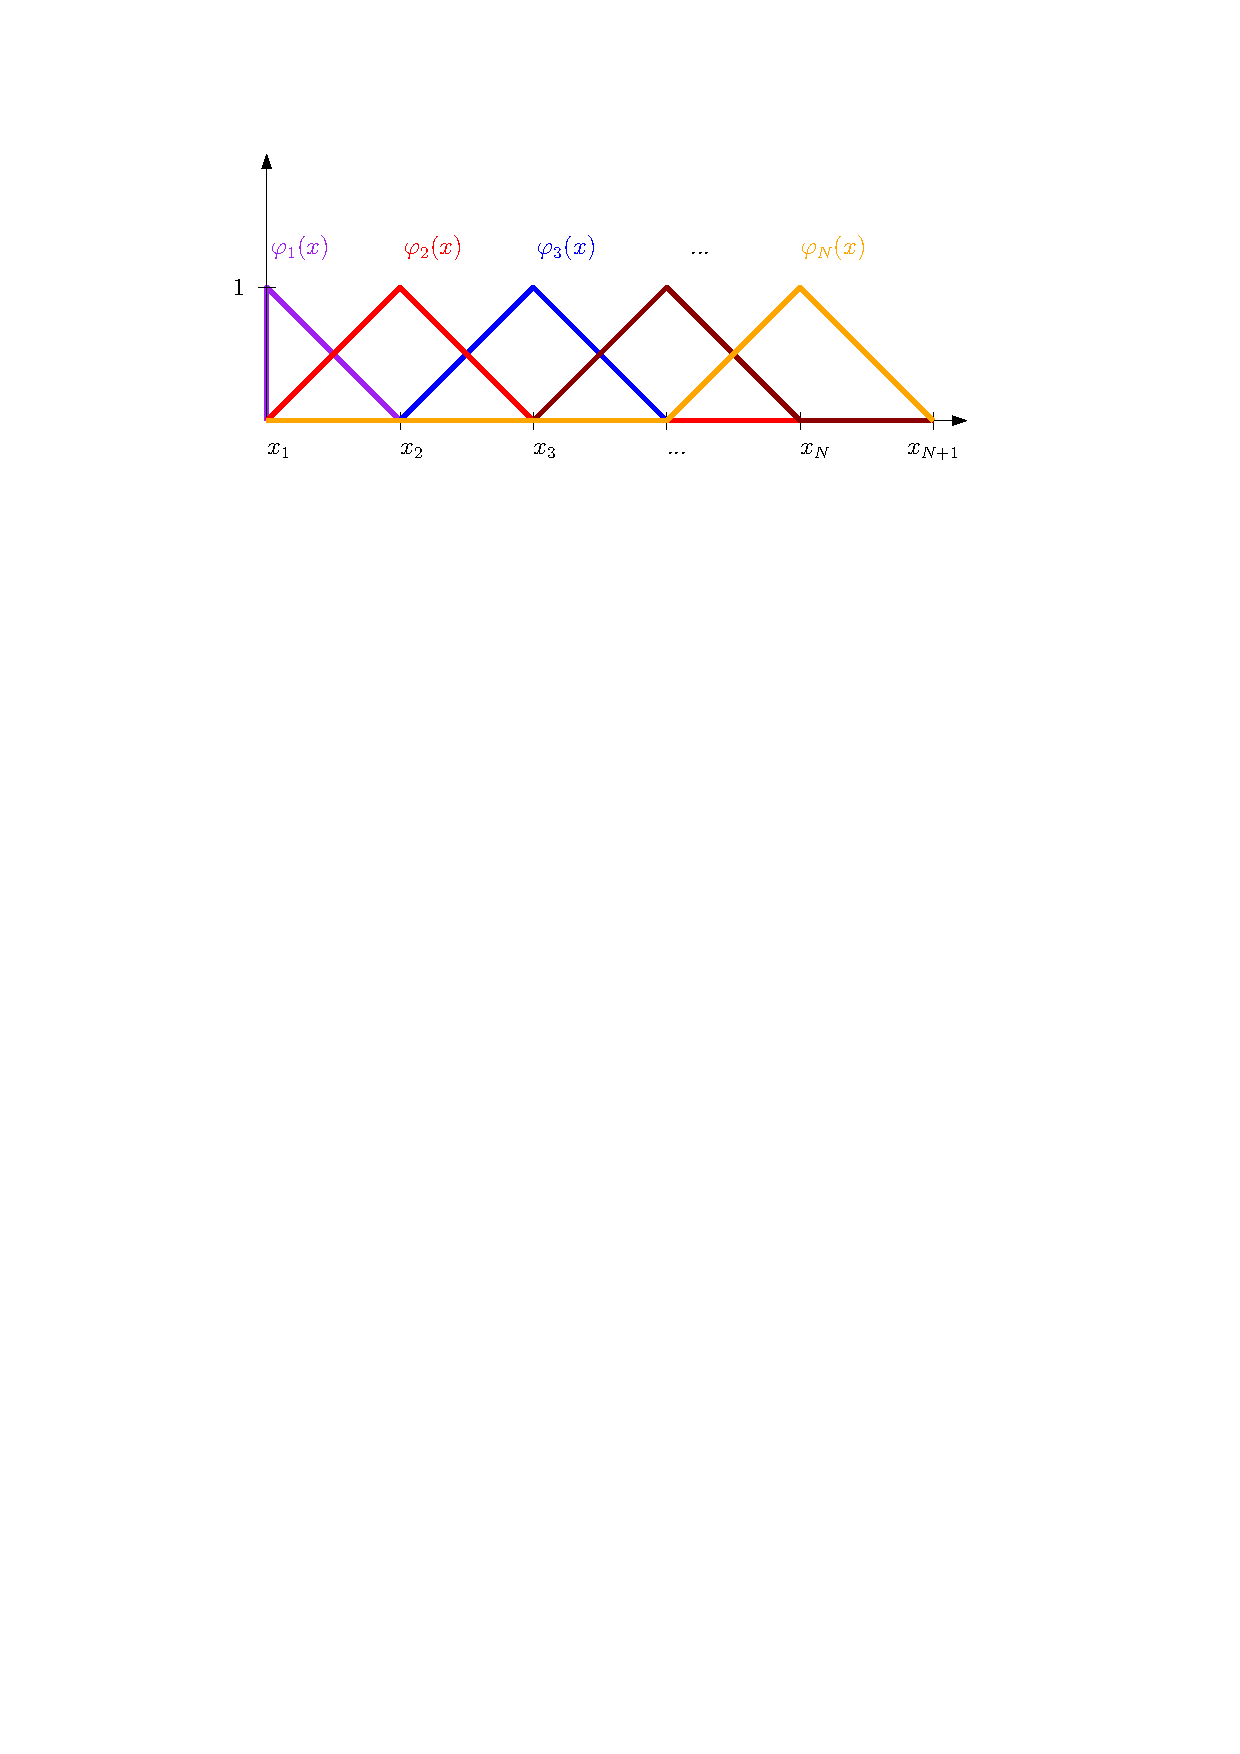
\includegraphics{base_1d_lin_termoska}
% \caption{Bázové funkce pro prostor po částech lineárních funkcí.}
% \label{fig:base_1d_lin}
% \end{figure}
% % Prvky matice $\tn A\in\R^{N\times N}$ a vektoru $\vc b\in\R^{N}$ mají tvar
% % \[ a_{ij}=\int_0^1\varphi_j'(x)\varphi_i(x), \]
% % \[ b_i = \int_0^1 f(x)\varphi_i(x)\d x. \]
% 
% Podívejme se nyní na konkrétní soustavu rovnic, kterou dostáváme z~\eqref{eqn:discrete_weak_form}.
% Je zřejmé, že $A_{ij}$ je nulové, pokud se indexy $i$ a $j$ liší více než o 1, neboť v takovém případě je v každém bodě intervalu $(0,1)$ alespoň jedna z funkcí $\varphi_i$, $\varphi_j$ (a tedy i $\varphi_i'$, $\varphi_j'$) nulová. Matice $\vc A$ proto bude třídiagonální, a tedy řídká.
% 
% Pokud budeme uvažovat $K(x) = const.\, \forall x\in E_j,\, j = 1\ldots N$, pak platí:
% \begin{align*}
% A_{jj} &= \int_{x_{j-1}}^{x_j} K(x)\varphi_j'(x)^2\d x + \int_{x_j}^{x_{j+1}} K(x) \varphi_j'(x)^2\d x
% = \int_{x_{j-1}}^{x_j}\frac{K}{h_{j-1}^2}\d x + \int_{x_j}^{x_{j+1}}\frac{K}{h_j^2}\d x\\
% &= K\left(\frac1{h_{j-1}} + \frac1{h_j}\right),~j=2,...,N,\\\\
% A_{11} &= \int_{x_1}^{x_{2}} K(x) \varphi_1'(x)^2\d x
% = \frac{K}{h_1},&\\\\
% A_{j,j-1} &= A_{j-1,j} = \int_{x_{j-1}}^{x_j}K(x)\varphi_{j-1}'(x)\varphi_j'(x)\d x\\
% &= \int_{x_{j-1}}^{x_j}\frac{(-K)}{h_{j-1}^2} \d x = -\frac{K}{h_{j-1}}, j=2,...,N.\\\\
% b_j &= \int_{x_{j-1}}^{x_{j+1}} f(x)\varphi_j(x)\d x,~j=2,...,N,&\\\\
% b_1 &= \int_{x_1}^{x_2} f(x)\varphi_1(x)\d x,&\\\\
% \end{align*}
% V případě ekvidistantního dělení ($h=h_j$ $\forall j=1,...,N$) a $K(x) = const.,\,f(x)=const.\, \forall x\in\Omega$ máme
% \[
%   \vc A = \frac{K}{h}\begin{pmatrix}1 & -1 &&& \\-1 & 2 & -1&&\\&\ddots&\ddots&\ddots&\\&&-1 & 2 & -1\\&&& -1 & 2\end{pmatrix}
%   = fh\begin{pmatrix}0.5\\1\\1\\1\\1\end{pmatrix}= \vc b.
% \]
% % Protože bilineární forma $(a,u,v)$ je symetrická a eliptická, je také $\tn A$ symetrická a pozitivně definitní.
% Soustava $\vc A\vc u_h=\vc b$ má řešení pro každý vektor $\vc b$,
% %a řešením Galerkinovy úlohy je funkce $u_h(x):=\sum_{i=1}^N\xi_i\varphi_i(x)$.
% hodnoty $u_h^i$ jsou zároveň hodnotami funkce $u_h$ v bodech $x_i$.
% 
% 
% \subsection{Chyba řešení}
% 
% Nyní budeme zkoumat chybu řešení, tedy v jakém vztahu jsou $u$ a $u_h$.
% Předem zavedeme zjednodušené značení
% \[
% a(u,v) = \int\limits_\Omega K(x) u'(x) v'(x) \d x, \qquad b(v) = \int\limits_\Omega f(x) v(x) \d x
% \]
% Nyní dosadíme $u$ a $u_h$ do naší slabé formulace, za použité nového značení a obě rovnice odečteme:
% \[
% \int\limits_\Omega K(x) u'(x) \varphi'(x) \d x = a(u,\varphi) = b(\varphi) = \int\limits_\Omega f \varphi(x) \d x
% \]
% \[
% \int\limits_\Omega K(x) u'(x) \varphi'(x) \d x = a(u,\varphi) = b(\varphi) = \int\limits_\Omega f \varphi(x) \d x
% \]
% 
% 
% 
% Podobně jako ve Větě \ref{th:cea} lze ukázat, že platí odhad chyby
% \begin{equation}\label{eq:error_est_laplace_dir}
% \forall v_h\in V_h:~\norm{u'-u_h'}_2 \le \norm{u'-v_h'}_2,
% \end{equation}
% takže $u_h$ je zároveň nejlepší aproximace slabého řešení $u$ v prostoru po částech lineárních funkcí.
% Zvolme nyní vhodnou funkci $v_h$, abychom odhad chyby \eqref{eq:error_est_laplace_dir} vyjádřili kvantitativně.
% Položíme $v_h:=\tilde u_h$, kde $\tilde u_h$ je interpolanta $u$ (po částech lineární funkce taková, že $\tilde u_h(x_i)=u(x_i)$, $i=0,...,N+1$).
% Pak z teorie Lagrangeovy interpolace víme, že platí
% \[ |u'(x)-\tilde u_h'(x)|\le h\max_{y\in[0,1]}|u''(y)| ~\forall x\in[0,1]. \]
% Je-li funkce $u$ třídy $C^2([0,1])$, pak dostáváme odhad
% \[ \norm{u'-u_h'}_2 \le \norm{u'-\tilde u_h'}_2 \le h\max_{y\in[0,1]}|u''(y)|, \]
% který říká, že chyba Galerkinovy aproximace měřená jako $L^2$ norma rozdílu derivací je řádu $O(h)$.
% 
% 
% 
% %\section{Rovnice vedení tepla}
% 
% 
% 
% % Uvažujme transportní rovnici na nekonečné oblasti $\Omega = \Real$ (pro $x$):
% % \begin{equation}
% %     \label{eq:point_transport_1d}
% %     \prtl_t u(t,x) + v\prtl_x u(t,x) =0 
% % \end{equation}
% % kde $v$ je konstantní rychlost. Řešením je posunutá počáteční podmínka $u_0(x)$:
% % \[
% %     u(t,x) = u_0(x-vt)
% % \]
% % pro libovolnou diferencovatelnou funkci $u_0$ máme:
% % \[
% %     \prtl_t u + v\prtl_x u=u_0'(x-vt)(-v) + vu_0'(x-vt)=0
% % \]
% % 
% % Zdá se logické, že by toto mělo platit pro libovolnou počáteční podmínku $u_0$, ale rovnice je formulována tak, že 
% % to platí jen pokud je $u_0$ diferencovatelná. Zkusme se vrátit k tomu jak jsme transportní rovnici odvodili. Pomocí Raynoldsovy věty jsme dostali:
% % \[
% %     \int_{\Omega_t} \prtl_t u + \div(v u) \d x= \int_{\Omega_t} \prtl_t u + v\prtl_x u \d x= 0
% % \]
% % pro libovolnou oblast $\Omega_t$. A bodovou rovnici \eqref{eq:point_transport_1d} jsme dostali za předpokladu, že vnitřek integrálu je spojitý, 
% % tedy $u$ je spojitě diferencovatelná v prostoru i čase. Tedy požadavek na diferencovatelnost je ve skutečnosti umělý a i bez něj platí:
% % \[
% %     \int_\Real \phi(\prtl_t u + \prtl_x(vu)) \d x = 0
% % \]
% % pro libovolnou hladkou funkci $\phi$ s kompaktním nosičem. Nosič funkce je množina, kde je funkce nenulová:
% % \[
% %     \supp \phi = \{ x,\ \phi(x) > 0\}
% % \]
% % a v našem případě jsou kompaktní všechny omezené a uzavřené intervaly. Jde tedy o to, že $\phi$ musí být \emph{směrem k nekonečnu} nulová.
% % 
% % Nyní však nevíme co je $\prtl_t u$ pokud je $u_0$ nespojitá, např. $u_0(x)=\sgn(x)$. Abychom se tohoto problému zbavili použijeme Greenovu větu 
% % (zde vlastně jen integraci per partes):
% % 
% % \[
% %     \int_\Real \int_\Real \phi(t,x)\big(\prtl_t u + \prtl_x(vu)\big) \d x \d t= 
% %     \int_\Real \int_\Real -\prtl_t \phi u - \prtl_x \phi vu \d x \d t = 0
% % \]
% % pro libovolnou hladkou funkci $\phi(t,x)$ s kompaktním nosičem na $\Real \times \Real$.
% % Tato rovnice již skutečně platí pro libovolnou integrovatelnou počáteční podmínku $u_0$.
% 
% 
% 
% 
% 
% 
\hypertarget{sec:diff_eq}{%
\section{MKP pro eliptické rovnice v 1D}
\label{sec:diff_eq}}

% \subsection{Motivace k~zavedení metody konečných prvků}
% 
% Řadu fyzikálních, chemických. biologických a sociálních procesů lze 
% popsat pomocí parciálních diferenciálních rovnic (PDR) a jejich soustav.
% Možnost řešení těchto rovnic je zásadní pro predikci a optimalizaci 
% příslušných procesů při řešení řady inženýrských problémů. PDR jsou rovnice, kde neznámou 
% je fyzikální pole popsané funkcí $u(\vc x)$, která bodům $\vc x$ 
% na na nějaké prostorové oblasti přiřazuje hodnoty pole. 
% Pro většinu PDR nelze řešení (funkci) zapsat v uzavřeném tvaru (t.j. vzorečkem) proto 
% jsou využány numerické (přibližné) metody jejichž výsledkem je funkce splňující rovnici 
% s nějakou numerickou chybou. Je to obdobné jako nemožnost reprezentovat v počítači přesně reálná čísla.
% 
% Metoda konečných prvků -- MKP, anglicky Finite Elment Method (FEM) je jednou ze standarodních metod pro numerické (přibližné)
% řešení PDR, dalšími metodamy jsou například metoda konečných objemů (Finite Volume Method -- FVM) 
% nebo nespojitá Galerkinova metoda (Discontinuous Galerkin -- DG).
% Společným rysem těchto metod je využití takzvané slabé formulace zadané rovnice. 
% V této kapitole si celý postup metody konečných prvků představíme na jednoduché úloze vedení tepla v 1D.

\subsection{Fyzikální úloha a klasická formulace}

\paragraph{Rozložení tepla v tělese.}
Příkladem úlohy popsané pomocí \emph{obyčejné diferenciální rovnice} (ODR) je rozložení teploty v tyči,
která je nějakým způsobem zahřívána. V~tomto případě nebudeme uvažovat tloušťku
tyče (předpokládáme, že teplota v příčném směru je konstantní) a počítáme tedy pouze v~1D souřadném systému. Jediná souřadnice je
$x\in[0,L]$ a interval $[0,L]$ představuje tyč o délce $L$. Teplotu v~různých částech tyče můžeme popsat funkcí
$u(x)$. Rovnice vedení tepla má tvar
\eq{\label{eq:heat_1d} -(k(x)u'(x))' = 0 \mbox{ pro }x\in(0,L), }
kde $k(x)$ je koeficient tepelné vodivosti v tyči (může být konstantní, pokud je materiál tyče homogenní). Výraz $-k(x)u'(x)$ představuje tepelný tok (úbytek tepla v bodě $x$).
% 
Rovnice \eqref{eq:heat_1d} popisuje rozložení tepla uvnitř tělesa.
Aby byl popis kompletní a matematická úloha řešitelná, je třeba upřesnit chování na hranici, tj. na koncích tyče.
Těmto vztahům říkáme \emph{okrajové podmínky}. Mezi nejběžnější typy okrajových podmínek pro rovnici vedení tepla patří:
\begin{enumerate}
\item[a)] Neumannova podmínka: Pokud je např. levý konec tyče zahříván vnějším zdrojem tepla s určitým tepelným tokem $g$, platí
\[ -k(0)u'(0)n(0) = g, \]
kde $n(x)$ je tzv. vnější jednotková normála nabývající hodnot $n(0)=-1$, $n(L)=1$ ($n$ určuje směr ``ven z tyče'').
Například hodnota $g=0$ znamená, že konec tyče je tepelně izolovaný od vnějšího prostředí.

\item[b)] Dirichletova podmínka: Pokud je pravý konec tyče udržován při konstantní teplotě $u_D$, platí
\[ u(L) = u_D. \]
\end{enumerate}

Taková úloha jde zobecnit i pro více dimenzí, můžeme např. popisovat
teplotu na nějaké dvourozměrné ploše (viz obr. \ref{fig:heat}).
\begin{figure}
\centering
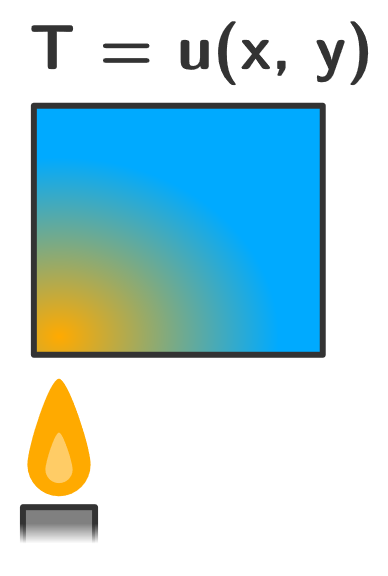
\includegraphics[width=0.3\textwidth]{img/image3.png}%
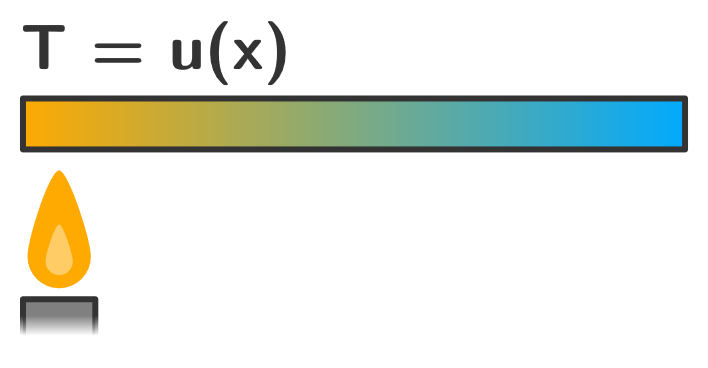
\includegraphics[width=0.5\textwidth]{img/image5.png}
\caption{Ilustrace fyzikální úlohy vedení tepla v rovinné oblasti (vlevo) a v 1D tyči (vpravo).}
\label{fig:heat}
\end{figure}
K~tomu bychom využili funkci
$u(x, y)$. Příslušná rovnice pak obsahuje derivace podle $x$ i
podle $y$. Takováto úloha ve více dimenzích s~derivacemi podle více
proměnných vede na využití \emph{parciálních diferenciálních rovnic}.
Okrajové úlohy pro ODR lze považovat za speciální případ (nejjednodušší) PDR.


\paragraph{Průhyb nosníku.}
Podobným způsobem lze matematicky popsat průhyb zatíženého nosníku.
Je-li tloušťka nosníku výrazně menší než jeho délka, pak lze nosník opět reprezentovat jako interval $[0,L]$.
Průhyb pak popisuje funkce $u(x)$, která splňuje rovnici bilance sil:
\[ -(k(x)u'(x))' = f(x) \mbox{ pro }x\in(0,L), \]
kde $k(x)$ je koeficient tuhosti materiálu nosníku a $f(x)$ je vnější objemová síla (zatížení působící po celé délce nosníku).
Výraz $k(x)u'(x)$ pak představuje vnitřní napětí v bodě $x$.
Podle toho, jak jsou upevněny konce nosníku je rovnice doplněna o okrajové podmínky. Např.:
\begin{enumerate}
\item[a)] Dirichletova podmínka: Je-li levý konec nosníku pevně uchycen, platí
\[ u(0)=0. \]
\item[b)] Neumannova podmínka: Je-li pravý konec nosníku zatížen, platí
\[ -k(L)u'(L)n(L) = g, \]
kde $g$ je vnější povrchová síla (zatížení působící v bodě $x=L$).
\end{enumerate}

\subsection{Klasická formulace okrajové úlohy}
Předchozí dva příklady fyzikálních problémů jsme popsali jako tzv. okrajové úlohy, sestávající z ODR a okrajových podmínek.
V další části budeme pracovat s okrajovou úlohou samostatně, bez přímé návaznosti na fyzikální problém.
Uvažujme tedy následující úlohu:
\begin{subequations}\label{eq:okr_uloha}
\begin{eqnarray}
-(k(x)u'(x))' &= f(x), &x\in(0,L),\label{eq:poisson}\\
-k(0)u'(0)n(0) &= g,\label{eq:neumann}\\
u(L) &= 0.\label{eq:hom_dirichlet}
\end{eqnarray}
\end{subequations}
Klasickým řešením úlohy \eqref{eq:okr_uloha} je funkce $u:[0,L]\to\Real$, která je dvakrát spojitě diferencovatelná a v příslušných bodech $x$ splňuje rovnice \eqref{eq:okr_uloha}.

\begin{ex}
Za speciálních zjednodušených podmínek je možné klasické řešení spočítat nebo ``uhodnout''.
Např. pokud $k(x)=f(x)=1$, $L=1$, $g=1$, pak klasické řešení má tvar
\[ u(x) = -\frac12(1-x)^2. \]
\end{ex}

Pro obecný případ s nekonstantními koeficienty se klasické řešení obvykle nedá vyjádřit v uzavřeném tvaru, tj. jako vzorec sestávající z aritmetických operací a analytických funkcí.
Proto je nutné hledat řešení přibližné (numerické).
To je předmětem metody konečných prvků.
Výchozí bod MKP je tzv. slabá formulace, jejíž odvození si ukážeme v následující sekci.


\subsection{Slabá formulace}

Slabou formulaci úlohy \eqref{eq:okr_uloha} získáme následujícím postupem.
\begin{enumerate}
\item Rovnici \eqref{eq:poisson} přenásobíme tzv. testovací funkcí $v(x)$, která splňuje Dirichletovu podmínku \eqref{eq:hom_dirichlet}, tj. $v(L)=0$:
\[ -(k(x)u'(x))'v(x) = f(x)v(x). \]

\item Vzniklou rovnici integrujeme přes interval $[0,L]$:
\[ \int_0^L -(k(x)u'(x))'v(x) \d x = \int_0^L f(x)v(x) \d x. \]

\item Levou stranu upravíme pomocí pravidla per partes:
\[ \int_0^L -(k(x)u'(x))'v(x) \d x = \left[-k(x)u'(x)v(x)\right]_{x=0}^L + \int_0^L k(x)u'(x)v'(x) \d x. \]

\item Aplikujeme okrajové podmínky:
\[ \left[-k(x)u'(x)v(x)\right]_{x=0}^L = -k(L)u'(L)\underbrace{v(L)}_{=0} + \underbrace{k(0)u'(0)}_{=g}v(0) = gv(0). \]
První člen je nahrazen díky volbě testovací funkce $v$ a druhý díky Neumannově okrajové podmínce.

\item Výsledná slabá formulace zní: Hledáme funkci $u\in V$, kde
\[ V=\{v:[0,L]\to\Real;~v \mbox{ je po částech diferencovatelná},~v(L)=0\}, \]
která splňuje
\eq{\label{eq:weak_poisson}
  \forall v\in V:\quad \int_0^L k(x)u'(x)v'(x) \d x = \int_0^L f(x)v(x) \d x - gv(0).
}
\end{enumerate}


Všimněme si dvou vlastností slabé formulace:
\begin{itemize}
  \item $u''$ nemusí existovat,
  \item $u'$ nemusí být spojitá, stačí existence integrálu na levé straně \eqref{eq:weak_poisson}.
\end{itemize}



\subsection{Galerkinova aproximace}
Nyní zvolíme konečně rozměrný vektorový podprostor $V_h\subset V$.
V tomto prostoru definujeme bázi $\{\varphi_j(x)\}_{j=1}^N$.
Tedy pro každou funkci $v_h\in V_h$ existuje právě jeden vektor $v_h^j,\, j=1\ldots N$,
takový že 
\[
  v_h(x) = \sum\limits_{j=1}^N v_h^j \varphi_j.
\]
% 
Uvažujme nyní aproximativní řešení $u_h\in V_h$ ve tvaru
\[
  u_h(x) = \sum\limits_{j=1}^N ´\xi^j \varphi_j.
\]
% 
Hledáme tedy $\vc\xi$ (vektor  koeficientů lineární kombinace), splňující \eqref{eq:weak_poisson} s testovacími funkcemi $v_h=\varphi_i$, $i=1,...,N$:
\eq{
  \int_0^L k(x) \left( \sum\limits_{j=1}^N \xi^j \varphi_j(x) \right)' \varphi_i'(x) \d x
    = \int_0^L f(x) \varphi_i(x) \d x - g\varphi(0)\qquad \forall i=1\ldots N \label{eqn:discrete_weak_form}
}
% 
Označíme-li
\[ a_{ij} := \int_0^L k(x) \varphi'_j(x) \varphi_i'(x) \d x, \]
\[ b_i := \int_0^L f(x) \varphi_i(x) \d x, \]
pak \eqref{eqn:discrete_weak_form} lze zapsat jako soustavu lineárních rovnic pro neznámý vektor $\vc\xi$:

\begin{equation}
  \mat A \vc\xi = \vc b\label{eqn:linear_system}
\end{equation}

Uveďme si nyní dvě zásadní vlastnosti matice $\mat A$, a to symetrii
\begin{equation}
  a_{ij} = \int_0^L k(x) \varphi'_j(x) \varphi_i'(x) \d x = \int_0^L k(x) \varphi'_i(x) \varphi_j'(x) \d x = a_{ji}, \label{eqn:linear_system_symetry}
\end{equation}
a pozitivní definitnost
\begin{multline}
  \vc\alpha^T \mat A \vc\alpha = \sum\limits_{i,j=1}^N \alpha_i \alpha_j a_{ij}
  = \int_0^L k(x)
    \underbrace{\left( \sum\limits_{i=1}^N \alpha_i \varphi'_i(x) \right)}_{\vc v}
    \underbrace{\left( \sum\limits_{j=1}^N \alpha_j \varphi'_j(x) \right)}_{\vc v} \d x \\
  = \int_0^L k(x) |\vc v|^2 > 0 \quad \forall \vc v: |\vc v|\neq 0. \label{eqn:linear_system_pos_def}
\end{multline}
    
    
    
\subsection{Lineární konečné prvky v 1D}
Jako podprostor $V_h$ zvolíme množinu lineárních lomených funkcí na intervalu $[0,L]$.
Rozdělme interval $[0,L]$ pomocí bodů $x_1=0<x_2<...<x_{N+1}=L$ na intervaly $E_j:=(x_j,x_{j+1})$ o délce $h_j:=x_{j+1}-x_{j}$.
Normu tohoto dělení zavedeme jako $h:=\max\limits_{j=1,...,N} h_j$.
Definujeme
\[ V_h:=\{v_h\in C([0,L]);~\forall j=1,...,N:~v_h \mbox{ je lineární na }E_j,~v_h(L)=0 \}. \]
%Jelikož funkce z $V_h$ jsou spojité a nulové v bodech $0$ a $1$, je automaticky $V_h$ podprostorem $H^1_0(0,1)$.
Každou funkci $v_h$ z $V_h$ jednoznačně určují její hodnoty v dělících bodech $\{x_j\}_{j=1}^N$.
Dimenze podprostoru tedy je $\dim V_h=N$.

Pro metodu konečných prvků je klíčová volba báze.
Zvolíme bázové funkce $\{\varphi_j\}_{j=1}^N$ podprostoru $V_h$ pomocí vztahů
\begin{equation*}
      \varphi_i(x_j) = 
        \begin{cases}
          1 \quad \textrm{pro } i=j\\
          0 \quad \textrm{pro } i\neq j\\
        \end{cases}
\end{equation*}
Každá bázová funkce je tedy nenulová v právě jednom uzlovém bodě (viz Obr. \ref{fig:base_1d_lin}). Všimněme si zde také, že na konci s Neumannovou okrajovou podmínkou existuje na intervalu $E_1$ funkce $\varphi_1$. Naopak na konci s Dirichletovou okrajovou podmínkou na intervalu $E_N$ existuje již pouze funkce $\varphi_N$. Prostory $V$ a $V_h$ a jejich báze závisí na konkrétních okrajových podmínkách.
\begin{figure}[h]
\centering
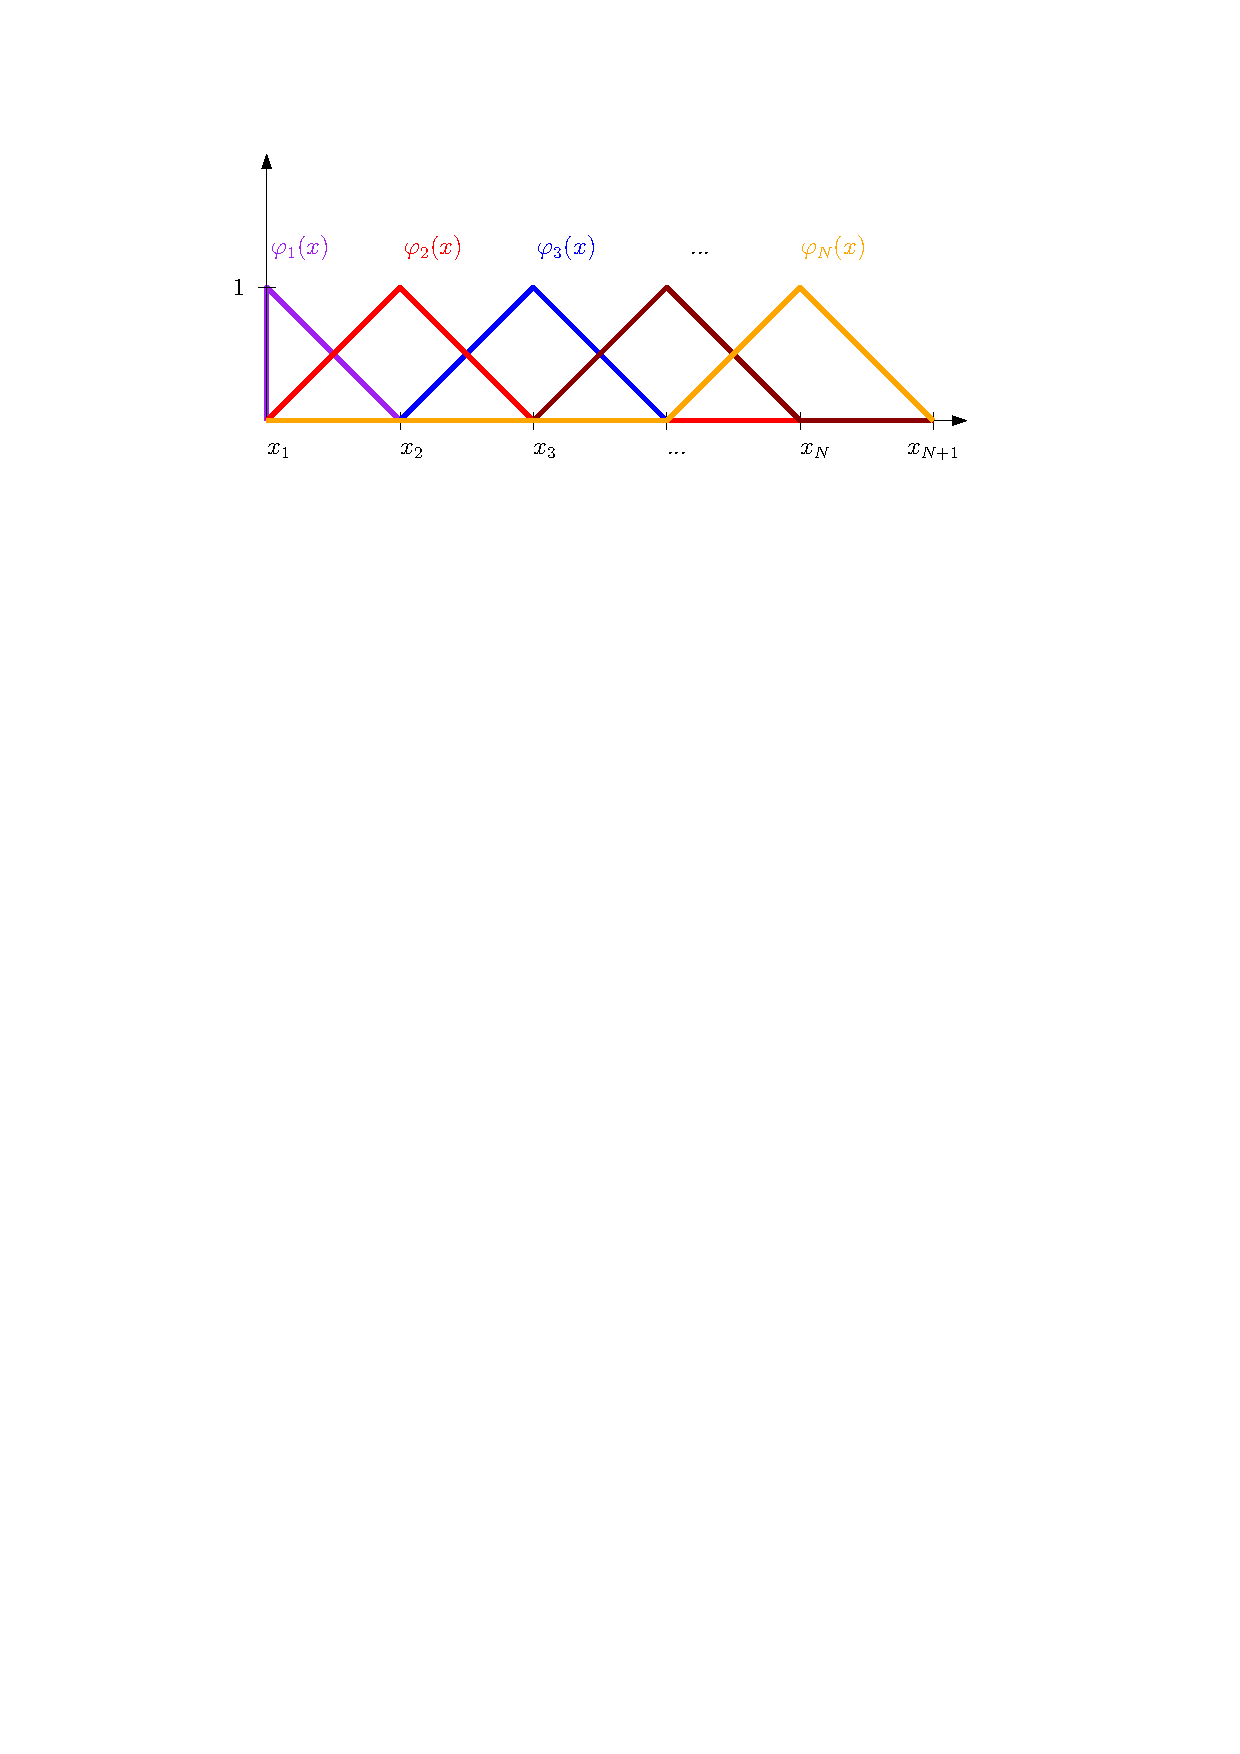
\includegraphics{base_1d_lin_termoska}
\caption{Bázové funkce pro prostor po částech lineárních funkcí.}
\label{fig:base_1d_lin}
\end{figure}
% Prvky matice $\tn A\in\R^{N\times N}$ a vektoru $\vc b\in\R^{N}$ mají tvar
% \[ a_{ij}=\int_0^1\varphi_j'(x)\varphi_i(x), \]
% \[ b_i = \int_0^1 f(x)\varphi_i(x)\d x. \]

Podívejme se nyní na konkrétní soustavu rovnic, kterou dostáváme z~\eqref{eqn:discrete_weak_form}.
Je zřejmé, že $a_{ij}$ je nulové, pokud se indexy $i$ a $j$ liší více než o 1, neboť v takovém případě je v každém bodě intervalu $(0,L)$ alespoň jedna z funkcí $\varphi_i$, $\varphi_j$ (a tedy i $\varphi_i'$, $\varphi_j'$) nulová. Matice $\mat A$ proto bude třídiagonální, a tedy řídká.

Pokud budeme uvažovat $K(x) = const.\, \forall x\in E_j,\, j = 1\ldots N$, pak platí:
\begin{align*}
A_{jj} &= \int_{x_{j-1}}^{x_j} K(x)\varphi_j'(x)^2\d x + \int_{x_j}^{x_{j+1}} K(x) \varphi_j'(x)^2\d x
= \int_{x_{j-1}}^{x_j}\frac{K}{h_{j-1}^2}\d x + \int_{x_j}^{x_{j+1}}\frac{K}{h_j^2}\d x\\
&= K\left(\frac1{h_{j-1}} + \frac1{h_j}\right),~j=2,...,N,\\\\
A_{11} &= \int_{x_1}^{x_{2}} K(x) \varphi_1'(x)^2\d x
= \frac{K}{h_1},&\\\\
A_{j,j-1} &= A_{j-1,j} = \int_{x_{j-1}}^{x_j}K(x)\varphi_{j-1}'(x)\varphi_j'(x)\d x\\
&= \int_{x_{j-1}}^{x_j}\frac{(-K)}{h_{j-1}^2} \d x = -\frac{K}{h_{j-1}}, j=2,...,N.\\\\
b_j &= \int_{x_{j-1}}^{x_{j+1}} f(x)\varphi_j(x)\d x,~j=2,...,N,&\\\\
b_1 &= \int_{x_1}^{x_2} f(x)\varphi_1(x)\d x,&\\\\
\end{align*}
V případě ekvidistantního dělení ($h=h_j$ $\forall j=1,...,N$) a $K(x) = const.,\,f(x)=const.\, \forall x\in\Omega$ máme
\[
  \vc A = \frac{K}{h}\begin{pmatrix}1 & -1 &&& \\-1 & 2 & -1&&\\&\ddots&\ddots&\ddots&\\&&-1 & 2 & -1\\&&& -1 & 2\end{pmatrix}
  = fh\begin{pmatrix}0.5\\1\\1\\1\\1\end{pmatrix}= \vc b.
\]
% Protože bilineární forma $(a,u,v)$ je symetrická a eliptická, je také $\tn A$ symetrická a pozitivně definitní.
Soustava $\vc A\vc u_h=\vc b$ má řešení pro každý vektor $\vc b$,
%a řešením Galerkinovy úlohy je funkce $u_h(x):=\sum_{i=1}^N\xi_i\varphi_i(x)$.
hodnoty $u_h^i$ jsou zároveň hodnotami funkce $u_h$ v bodech $x_i$.


\subsection{Chyba řešení}

Nyní budeme zkoumat chybu řešení, tedy v jakém vztahu jsou $u$ a $u_h$.
Předem zavedeme zjednodušené značení
\[
a(u,v) = \int\limits_\Omega K(x) u'(x) v'(x) \d x, \qquad b(v) = \int\limits_\Omega f(x) v(x) \d x
\]
Nyní dosadíme $u$ a $u_h$ do naší slabé formulace, za použité nového značení a obě rovnice odečteme:
\[
\int\limits_\Omega K(x) u'(x) \varphi'(x) \d x = a(u,\varphi) = b(\varphi) = \int\limits_\Omega f \varphi(x) \d x
\]
\[
\int\limits_\Omega K(x) u'(x) \varphi'(x) \d x = a(u,\varphi) = b(\varphi) = \int\limits_\Omega f \varphi(x) \d x
\]



Podobně jako ve Větě \ref{th:cea} lze ukázat, že platí odhad chyby
\begin{equation}\label{eq:error_est_laplace_dir}
\forall v_h\in V_h:~\norm{u'-u_h'}_2 \le \norm{u'-v_h'}_2,
\end{equation}
takže $u_h$ je zároveň nejlepší aproximace slabého řešení $u$ v prostoru po částech lineárních funkcí.
Zvolme nyní vhodnou funkci $v_h$, abychom odhad chyby \eqref{eq:error_est_laplace_dir} vyjádřili kvantitativně.
Položíme $v_h:=\tilde u_h$, kde $\tilde u_h$ je interpolanta $u$ (po částech lineární funkce taková, že $\tilde u_h(x_i)=u(x_i)$, $i=0,...,N+1$).
Pak z teorie Lagrangeovy interpolace víme, že platí
\[ |u'(x)-\tilde u_h'(x)|\le h\max_{y\in[0,1]}|u''(y)| ~\forall x\in[0,1]. \]
Je-li funkce $u$ třídy $C^2([0,1])$, pak dostáváme odhad
\[ \norm{u'-u_h'}_2 \le \norm{u'-\tilde u_h'}_2 \le h\max_{y\in[0,1]}|u''(y)|, \]
který říká, že chyba Galerkinovy aproximace měřená jako $L^2$ norma rozdílu derivací je řádu $O(h)$.






% V~matematice a fyzice jsme se dosud v~souvislosti s~diferenciálními
% rovnicemi setkávali s~tzv. \textbf{počátečním problémem} neboli
% \textbf{úlohou s~počátečními podmínkami} (Cauchyho úlohou). Příkladem
% úlohy, kterou lze takto řešit je kyvadlo. To můžeme aproximovat jako
% lineární oscilátor a při zadaných počátečních podmínkách (počáteční
% výchylka) dokážeme pomocí ODR závislé pouze na čase (\emph{\textbf{t}})
% popsat časový vývoj tohoto systému až do nekonečna (např. až do
% zastavení kyvadla).

% \subsection{Okrajová úloha, typy okrajových podmínek}
% 
% 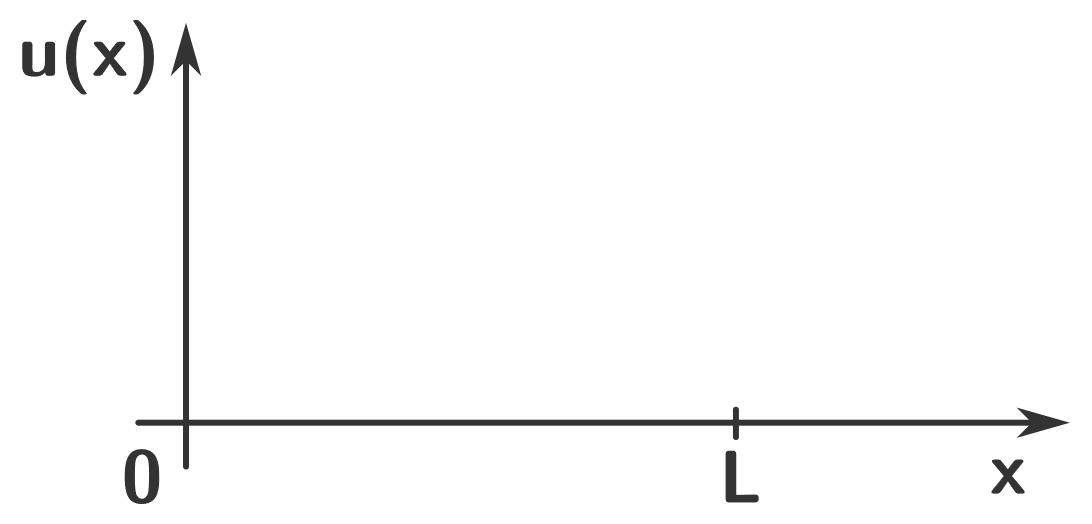
\includegraphics[width=1.93264in,height=0.92708in]{img/image7.png}
% 
% Jiný
% typ úlohy, kterým se zejména budeme zabývat, je tzv. \textbf{okrajová
% úloha}, kde máme zadané podmínky v~krajních bodech zkoumaného intervalu.
% Jako příklad použijeme výše zmíněnou úlohu s~teplotou tyče. Tyč má délku
% \emph{\textbf{L}} a rovnici popisující vývoj její teploty obecně
% zapíšeme jako:
% 
% \[- k  u^{''}\left( x \right) = f(x)\]
% 
% Kde \emph{\textbf{k}}~je konstanta, v~tomto případě \emph{koeficient
% tepelné vodivosti} a \emph{\textbf{f(x)}} je funkce popisující zdroj
% tepla s~fyzikálním rozměrem W/m (watt na metr). Existují dva typy
% okrajových podmínek, kterými se budeme zabývat, ukážeme si je na
% příkladech:
% 
% 1. typ -- Neumannova podmínka: Představme si, že tyč je na jednom konci
% (v bodě \(x\  = \ 0\)) izolována, takže z~ní nemůže unikat teplo do
% okolí. Tuto situaci lze matematicky zapsat jako:
% 
% \[u'\left( 0 \right) = 0\]
% 
% Přičemž 1. derivace \(u\) souvisí s~\textbf{tokem tepla}, který má
% obecně podobu \(- k \bullet u'\) a někdy se značí \(q\). Podmínka, která
% definuje \textbf{tok} nějaké veličiny v~okrajovém bodě se nazývá
% \textbf{Neumannova podmínka}.
% 
% 2. typ -- Dirichletova podmínka: Na druhém konci tyče (v bodě
% \(x\  = \ L\)) je termostat, který udržuje konstantní teplotu (např. 0
% °C). To lze zapsat jako:
% 
% \[u\left( L \right) = konst.\ (\text{např.}\ 0\ {^\circ}C)\]
% 
% Tento typ podmínky, který definuje \textbf{hodnotu} nějaké veličiny
% v~okrajovém bodě se nazývá \textbf{Dirichletova podmínka.}
% 
% \[- k \bullet u^{''}\left( x \right) = f(x)\]
% 
% V~tomto případě označuje \emph{\textbf{k}}~tuhost nosníku a funkce
% \emph{f} nějakým způsobem vyjadřuje sílu či zatížení seshora. Takto lze
% vymyslet ještě mnoho dalších úloh popsatelných stejnou rovnicí (např.
% šíření chemické látky nějaké koncentrace uzavřeným systémem).
% 
% Slabá formulace problému:
% 
% Rovnice \(- k \bullet u^{''}\left( x \right) = f(x)\) popisující uvedené
% úlohy byla dosud udávána v~tzv. \textbf{bodovém tvaru}, který se tak
% označuje, protože popisuje všechny body zkoumaného intervalu (např. u
% úlohy s~tyčí platí pro všechna \emph{x} z~intervalu (0, \emph{L})).
% Fyzikálně vychází tato rovnice ze zákona zachování energie (kolik
% energie ve formě tepla do tyče přiteče, tolik musí i odtéct), konkrétně
% u úloh o teplu z~Fourierova zákona, který popisuje závislost toku tepla
% na gradientu teploty. Tato fyzikální interpretace nemá bodový, ale
% \textbf{integrální} charakter (gradient popisuje změny při nekonečně
% malém posunutí, integrací lze poté popisovat celý zkoumaný objekt).
% Integrální tvar, také nazývaný \textbf{slabá formulace}, je vhodný i pro
% numerické řešení těchto úloh, využívající metodu konečných prvků.
% Dostaneme se k~němu postupnou úpravou dříve zkoumané diferenciální
% rovnice (zde jsou derivace zapsány obecněji, protože i \(k\)~může
% záviset na \(x\)):
% 
% \[- \left( ku^{'} \right)^{'}\left( x \right) = f(x)\]
% 
% Obě strany rovnice vynásobíme tzv. \textbf{testovací funkcí}
% \(\varphi(x)\), která může být libovolná, ale měla by být na celém
% intervalu (0, \emph{L}) nekonečně diferencovatelná (tak hladká a
% „pěkná``, že má ve všech bodech derivace všech řádů):
% 
% \[- \left( ku^{'} \right)^{'}\left( x \right) \bullet \varphi(x) = f(x) \bullet \varphi(x)\]
% 
% Následně obě strany rovnice integrujeme podle \emph{\textbf{x}} na
% intervalu od 0 do \emph{L}:
% 
% \[\int_{0}^{L}{- \left( ku^{'} \right)^{'}\left( x \right) \bullet \varphi(x)}dx = \int_{0}^{L}{f(x) \bullet \varphi(x)}\text{dx}\]
% 
% Poté integrál upravíme pomocí per partes (za funkce již nebudu psát, že
% jsou to funkce proměnné \emph{x}):
% 
% \[\left\lbrack - ku'\varphi \right\rbrack_{0}^{L} + \int_{0}^{L}{ku^{'}\varphi^{'}dx = \int_{0}^{L}{f\varphi}\text{dx}}\]
% 
% Nyní předpokládejme, že máme pro funkci zadané tyto okrajové podmínky
% (OKP):
% 
% První (levá strana):
% \(q\left( 0 \right) = - ku^{'}\left( 0 \right) = g\) kde \emph{q} značí
% tok a \emph{g} je nějaká konstantní hodnota
% 
% Druhá (pravá strana): u(L) = 0 (pro zjednodušení, obecně to může být
% libovolná hodnota, ale výpočty jsou pak složitější)
% 
% Také zatím předpokládáme, že pro zvolenou funkci \(\varphi(x)\)
% platí\(\text{\ phi}\left( L \right) = 0\), tím se příklad dále zjednoduší.
% S~těmito podmínkami a předpoklady rozepišme hranatou závorku, kterou
% jsme získali použitím per partes:
% 
% \[\left\lbrack - ku'\varphi \right\rbrack_{0}^{L} = q\left( L \right)\varphi\left( L \right) - q(0)\varphi(0)\]
% 
% \[\ \ \ \ \ \ \ \ \ \ \ \ \ \ \ \ \ \ \ \ \ \ \ \ \ \ \ \  = 0\ \ \ \ \ \ \ \ \ \ \ \  = g\varphi(0)\]
% 
% po dosazení zpět do rovnice dostaneme:
% 
% \[- g\varphi(0) + \int_{0}^{L}{ku^{'}\varphi^{'}dx = \int_{0}^{L}{f\varphi}\text{dx}}\]
% 
% Funkce \(u(x)\) se nazývá \textbf{slabé řešení}, pokud splňuje tyto
% podmínky:
% 
% \begin{enumerate}
% \def\labelenumi{\arabic{enumi}.}
% \item
%   \(u \in H^{1}(0,\ L)\) -- \(u\) je kvadraticky integrabilní na
%   intervalu od 0 do \emph{L} (tedy, první derivace \(u^{2}\) na celém
%   intervalu (0, \emph{L}) existuje a je konečná)
% \item
%   \(u\left( L \right) = 0\) -- musí být zadána tato Dirichletova
%   podmínka (to jsme udělali)
% \item
%   \(- g\varphi(0) + \int_{0}^{L}{ku^{'}\varphi^{'}dx = \int_{0}^{L}{f\varphi}\text{dx}}\)
%   platí pro všechny testovací funkce \(\varphi \in C^{\infty}(0,\ L)\)
% \end{enumerate}
% 
% 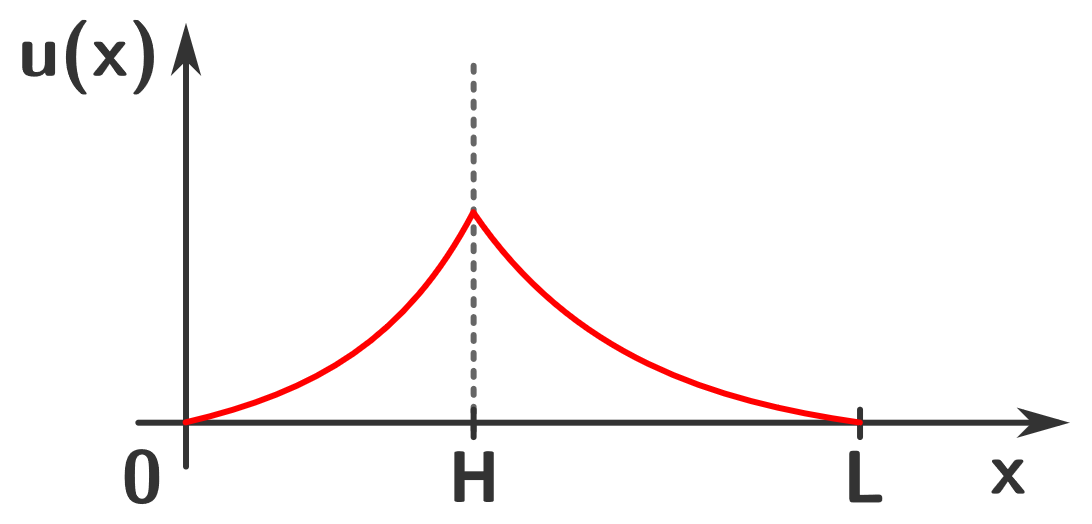
\includegraphics[width=2.36597in,height=1.13542in]{img/image11.png}Slabé
% řešení je obecnější než bodové řešení (bodové řešení, jak plyne již ze
% zápisu bodového tvaru, musí mít druhou derivaci, mohou však existovat
% slabá řešení, která tuto podmínku nesplňují). To lze ukázat na
% následujícím příkladě:
% 
% Pokud zahříváme tyč v~bodě \emph{H}, a máme zadáno, že na obou koncích
% je teplota 0 (příslušných jednotek), bude funkce \(u(x)\) vypadat jako
% na grafu vpravo. V~bodě \emph{H} je tato funkce ostrá a druhá derivace
% tam neexistuje. Bodové řešení tedy neexistuje. Přesto by k~této úloze
% šlo najít slabé řešení.
% 
% Platí, že pokud existuje bodové řešení, existuje i slabé řešení a obě
% tato řešení jsou shodná. Pokud má slabé řešení druhé derivace, je
% zaručeno, že existuje i bodové řešení. Bodovému řešení se také někdy
% říká \textbf{silné řešení}.
% 
% Finální tvar rovnice můžeme přepsat (zaměnit pořadí členů) takto:
% 
% \[\int_{0}^{L}{ku^{'}\varphi^{'}dx = \int_{0}^{L}{f\varphi}dx + g\varphi(0)}\]
% 
% poté se na pravé straně vůbec nevyskytuje funkce \(u\), pouze známé
% funkce a konstanty.
% 
% Galerkinova aproximace:
% 
% Často se stane, že řešení podobných diferenciálních rovnic, se kterými
% jsme doteď pracovali, nelze nalézt analyticky. V~takovém případě je
% nutné provést aproximaci, například pomocí polynomů.
% 
% Před pokračováním si zopakujme některé pojmy z~lineární algebry, které
% budeme používat:
% 
% \begin{itemize}
% \item
%   Konečněrozměrný vektorový prostor: prostor vektorů
%   \(\left( u_{1},\ u_{2},\ u_{3},\ \ldots,u_{n} \right) \in \mathbb{R}^{n}\).
%   Je na něm definováno sčítání a násobení skalárem, jejich výsledky leží
%   opět v~tom samém vektorovém prostoru.
% \item
%   Vektorový prostor funkcí: příkladem je prostor polynomů do
%   \emph{n}-tého řádu \(P^{n}\).
% \item
%   Dimenze vektorového prostoru: počet složek vektorů v~prostoru a
%   zároveň největší počet lineárně nezávislých vektorů, který může
%   v~prostoru existovat. \emph{n}-rozměrný vektorový prostor má dimenzi
%   \emph{n}, prostor polynomů do řádu \emph{n} má dimenzi \emph{n} + 1.
% \item
%   Lineární kombinace vektorů (polynomů, čehokoliv, \ldots{}):
%   \(\alpha_{1} \bullet v_{1}\left( x \right) + \alpha_{2} \bullet v_{2}\left( x \right) + \alpha_{3} \bullet v_{3}\left( x \right) + \ldots\)
%   kde \(\alpha_{i}\) jsou konstanty a \(v_{i}\) jsou vektory, polynomy,
%   obecně prvky daného prostoru.
% \item
%   Lineárně nezávislé vektory: Skupina vektorů z~nějakého prostoru,
%   z~nichž žádný nelze vytvořit jako lineární kombinaci těch ostatních.
% \item
%   Báze \emph{n}-rozměrného prostoru: \emph{n}-tice lineárně nezávislých
%   vektorů z~daného prostoru, takových, že každý vektor z~daného prostoru
%   lze vytvořit jako jejich lineární kombinaci. Např. pro prostor
%   polynomů \(P^{2}\) je nejjednodušší báze trojice \(1,\ x,\ x^{2}\),
%   lze však nalézt i jinou bázi.
% \end{itemize}
% 
% Galerkinova aproximace nám umožní s~využitím nějakého vektorového
% prostoru funkcí nalézt aproximované řešení úloh s~DR, které nelze nalézt
% analyticky. Začneme volbou báze \(\varphi_{1},\ \ldots,\ \varphi_{n}\).
% Řešení \(u_{h}(x)\) budeme hledat ve zvoleném prostoru funkcí. Víme, že
% každý vektor ze zvoleného prostoru lze zapsat jako lineární kombinaci
% bázových vektorů, platí tedy:
% 
% \[u_{h}\left( x \right) = \sum_{i = 1}^{n}{u_{i} \bullet \varphi_{i}\left( x \right)}\]
% 
% (pozor, \(u_{i}\) na pravé straně je zde skalár)
% 
% toto aproximativní řešení dosadíme do slabé formulace (využíváme
% testovací funkce \(\varphi_{j}\), kde \(j = 1,\ldots,\ n\), které nejsou
% shodné s~vektory báze \(\varphi_{i}\)):
% 
% \[\int_{0}^{L}{k\left( \sum_{i = 1}^{n}{u_{i} \bullet \varphi_{i})} \right)^{'}{\varphi_{j}}^{'}dx = \int_{0}^{L}{f\varphi_{j}}dx + q(0)\varphi_{j}(0)}\]
% 
% po úpravě:
% 
% \[\sum_{i = 1}^{n}{u_{i} \bullet}\left( \int_{0}^{L}{\text{kphi}_{i}'\varphi_{j}'} \right) = \overrightarrow{b}\]
% 
% kde vektor \(\overrightarrow{b}\) na pravé straně vznikl vyřešením
% integrálů na pravé straně, které daly \emph{n}-tici čísel
% \(b_{j}\)\emph{. Vyřešením integrálu v~závorce na levé straně dostaneme
% matici} \(A_{\text{ji}}\) a suma před integrálem vyprodukuje vektor
% \(\overrightarrow{u}\). Řešení tedy dostaneme ve tvaru:
% 
% \[\overrightarrow{u} \bullet A = \overrightarrow{b}\]
% 
% Pokud si vzpomeneme na lineární algebru, tento zápis vlastně znamená
% soustavu lineárních rovnic. Jejím vyřešením bychom našli neznámé
% koeficienty \(u_{i}\) \emph{a tedy i řešení} \(u_{h}(x)\). Přesnost této
% (Galerkinovy) aproximace závisí na zvoleném prostoru, ve kterým ji
% provádíme.
% 
% Metoda konečných prvků (MKP):
% 
% MKP je speciální případ Galerkinovy aproximace, kde volíme vektorový
% prostor a jeho bázi takovým způsobem, aby šlo aproximovat i funkce, ve
% kterých by se standardní Galerkinova aproximace mohla chovat nepříliš
% ideálně.
% 
% 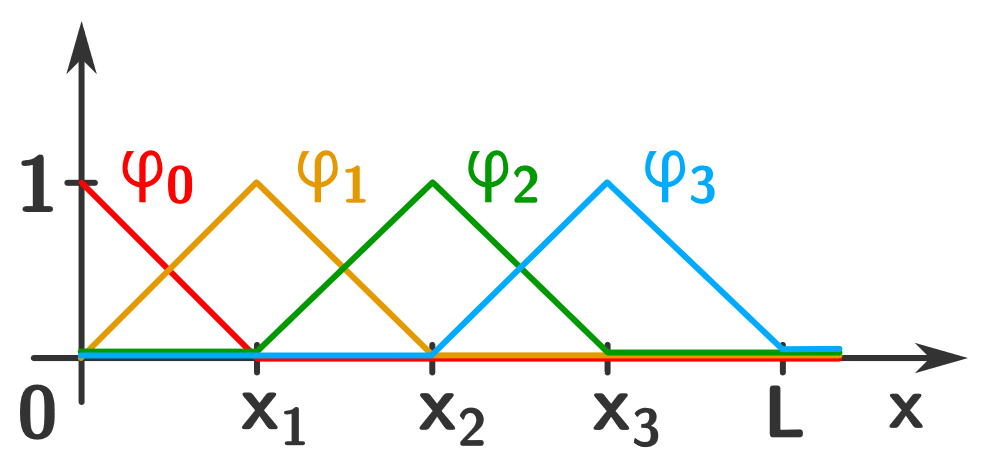
\includegraphics[width=2.72222in,height=1.28958in]{img/image13.png}Ke
% zvolení báze pro MKP si interval (0, \emph{L}) na kterém počítáme
% rozdělíme pomocí konečného počtu bodů \(x_{1},\ x_{2}\) atd na několik
% menších intervalů. Jako bázi poté zvolíme sadu funkcí, z~nichž se každá
% chová jako lineární polynomiální funkce jdoucí do 1 v~okolí jednoho
% z~bodů a v~okolí ostatních je nulová, viz graf napravo.
% 
% Výpočet integrálu, ze kterého vznikne matice A může být u~Galerkinovy
% metody komplikovaný, u MKP jsou však bázové vektory zvoleny tak
% „šikovně``, že matice je tzv. řídká neboli na hodně pozicích vyjde nula
% (protože součin \(\varphi_{i}'\varphi_{j}'\) vychází 0 pro funkce které
% jsou od sebe příliš „vzdálené``). To urychluje její výpočet a také
% usnadňuje ukládání dat do počítače -- jejich velikost je výrazně menší
% (u dostatečně přesných aproximací je někdy potřeba ukládat řádově až
% miliardy intervalů!):
% 
% \[A_{\text{ij}} = \int_{0}^{L}{\text{k\ phi}_{i}'\varphi_{j}'}\ dx = 0\ např.\ pro\text{\ phi}_{0}\ a\ \varphi_{2}\]
% 
% \begin{longtable}[]{@{}ll@{}}
% \toprule
% \endhead
% \begin{minipage}[t]{0.47\columnwidth}\raggedright
% \[A_{01} = \int_{x0}^{x1}{\text{k\ phi}_{0}'\varphi_{1}'} = 0\]
% 
% \[A_{02} = \int_{x0}^{x1}{\text{k\ phi}_{0}'\varphi_{1}'} = 0\]
% 
% \[A_{10} = \int_{x0}^{x1}{\text{k\ phi}_{1}'\varphi_{0}'} = A_{01}\]\strut
% \end{minipage} & \begin{minipage}[t]{0.47\columnwidth}\raggedright
% \[A_{11} = \int_{x0}^{x1}{\text{k\ phi}_{1}'\varphi_{1}'} + \int_{x1}^{x2}{\text{k\ phi}_{1}'\varphi_{1}'}\]
% 
% \[A_{12} = \int_{x1}^{x2}{\text{k\ phi}_{1}'\varphi_{2}'}\]
% 
% a tak dále\ldots{}\strut
% \end{minipage}\tabularnewline
% \bottomrule
% \end{longtable}
% 
% Matice vzniklá při aproximaci MKP má obecně následující podobu 
% ($\bullet$ a $\blacksquare$)
% značí nenulové hodnoty):
% 
% \[\begin{bmatrix}
% \bullet & \blacksquare & 0 & 0 & \cdots & 0 \\
% \blacksquare & \bullet & \blacksquare & 0 & \dots & \vdots \\
% 0 & \blacksquare & \bullet & \blacksquare & 0 & 0 \\
% 0 & 0 & \blacksquare & \bullet & \blacksquare & 0 \\
%  \vdots & \dots & 0 & \blacksquare & \bullet & \blacksquare \\
% 0 & \cdots & 0 & 0 & \blacksquare & \bullet \\
% \end{bmatrix}\]
% 
% Tedy jedna nenulová hodnota se opakuje na hlavní diagonále, jiná nad a
% pod ní, zbytek jsou nuly. Je zjevné, že pokud by taková matice měla
% rozměr třeba milion × milion, manipulovalo by se s~ní mnohem snadněji
% než se stejně velkou maticí, která by měla nenulové hodnoty všude.
% 
% Matice vzniklá aplikací MKP při řešení eliptických úloh (to jsou úlohy
% uváděné v~této kapitole jako příklad) je symetrická a pozitivně
% definitní.
% 
% Všechno je pochopitelně mnohem komplikovanější ve více dimenzích nebo
% v~reálnějších, ne tak „hezky`` zadaných případech. Jak se pomocí MKP
% reálně úlohy řeší bude náplní dalších přednášek.
% 
% \hypertarget{bilineuxe1rnuxed-forma-volba-podprostoru-vh-struktura-matice-a-07.10.2020}{%
% \section{\texorpdfstring{Bilineární forma, volba podprostoru
% \emph{V\textsubscript{h}}, struktura matice \emph{A}
% (07.10.2020)}{Bilineární forma, volba podprostoru Vh, struktura matice A (07.10.2020)}}\label{bilineuxe1rnuxed-forma-volba-podprostoru-vh-struktura-matice-a-07.10.2020}}
% 
% Příklad na shrnutí látky z~minulé přednášky:
% 
% 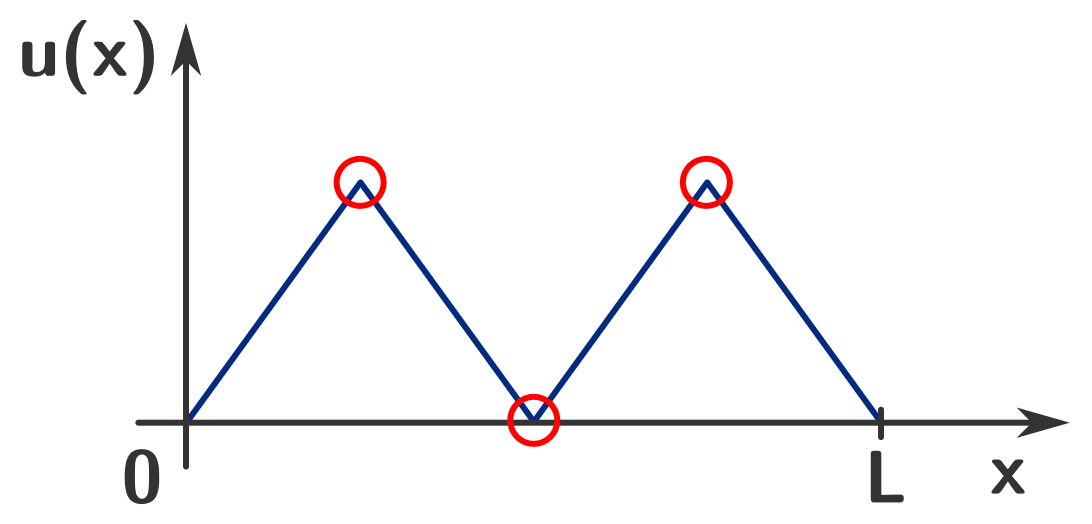
\includegraphics[width=2.84375in,height=1.36458in]{img/image15.png}Řešíme
% okrajovou úlohu zadanou rovnicí:
% \(- ku^{''}\left( x \right) = f\left( x \right)\). Pokud bychom
% uvažovali, že úloha se týká vedení tepla, poté \(k\)~odpovídá tepelné
% vodivosti, \(u(x)\) je teplota a \(f(x)\) je hustota tepelného zdroje.
% Známe také okrajové podmínky v~obou krajních bodech (0~a~\emph{L}).
% 
% Pokud chceme najít bodové řešení, musí být funkce u(x) dostatečně
% hladká, aby měla na celém intervalu (0, \emph{L}) druhé derivace. Např.
% u funkce vykreslené vpravo by byl problém v~červeně označených bodech.
% Můžeme však nalézt slabé řešení. Z~minula víme, že bude mít tvar:
% 
% \[\int_{0}^{L}{ku^{'}\varphi^{'}dx = \int_{0}^{L}{f\varphi}\text{dx}}{- \ \left\lbrack ku'\varphi \right\rbrack}_{0}^{L}\]
% 
% Máme zadané dvě okrajové podmínky, každou jiného typu:
% 
% \begin{enumerate}
% \def\labelenumi{\Roman{enumi}.}
% \item
%   Dirichletova podmínka: \(u(0) = 0\) (může být i nenulová hodnota, ale
%   to je složitější). Důsledkem této podmínky je zmenšení prostoru řešení
%   jen na určité funkce:
%   \(u \in \left\{ u \in H^{1}\left( 0,L \right),\ u\left( 0 \right) = 0 \right\}\)
%   -- \(u\)~může být jen funkce patřící do množiny \(H^{1}\) na intervalu
%   (0, \emph{L}), která je navíc v~bodě 0 nulová. (\(H^{1}\) je množina
%   funkcí které lze určitým způsobem alespoň jednou derivovat na (0,
%   \emph{L}), více o tomto později.). Množinu (vektorový prostor) funkcí
%   ze které pochází \(u\) označíme jako \(V\).
% \item
%   Neumannova podmínka: \(- ku^{'}\left( L \right) = g\) (\(- ku^{'}\) je
%   tok v~okrajovém bodě L). Tuto podmínku lze dosadit přímo do rovnice
%   slabé formulace.
% \end{enumerate}
% 
% Co nebylo minule zmíněno je, že testovací funkce \(\varphi\) musí
% pocházet ze stejného prostoru, jako funkce u, tedy v~tomto případě
% platí: \(\varphi \in V,\ \varphi\left( 0 \right) = 0\). Aplikací
% podmínek a této úvahy upravíme slabou formulaci do tvaru:
% 
% \[\int_{0}^{L}{ku^{'}\varphi^{'}dx = \int_{0}^{L}{f\varphi}\text{dx}} + g\varphi(L)\]
% 
% Tento vztah musí platit pro všechny testovací funkce \(\varphi \in V\).
% Prostor \(V\)~ve skutečnosti obsahuje i „zubaté`` funkce (jako na grafu
% výše) které nemají všude derivace, takové funkce však můžeme
% s~libovolnou přesností aproximovat hladkými funkcemi podobného tvaru. To
% však pouze, pokud má slabá formulace lineární strukturu \(\varphi\), což
% je zde splněno (derivace, násobení, integrál. jsou lineární operace --
% více o tomto později).
% 
% Pokud chceme provést Galerkinovu aproximaci, aproximujeme prostor \(V\),
% který má obecně nekonečnou dimenzi konečněrozměrným prostorem \(V_{h}\)
% (např. prostorem polynomů do určitého stupně), který je
% \textbf{podprostorem prostoru} \(\mathbf{V}\).
% 
% Protože \(V_{h}\) má konečnou dimenzi, lze v~něm nalézt také bázi. Tu
% tvoří funkce \(\varphi_{1}(x),\varphi_{2}(x),\ldots,\varphi_{n}(x)\).
% Galerkinova aproximace najde funkci \(u_{h}(x)\), která přibližně
% odpovídá funkci \(u(x)\) a dá se napsat jako lineární kombinace bázových
% funkcí prostoru \(V_{h}\):
% 
% \[u_{h}\left( x \right) = \sum_{i = 1}^{n}{u_{i} \bullet \varphi_{i}(x)}\]
% 
% K~určení aproximované funkce \(u_{h}\left( x \right)\) stačí znát
% koeficienty \(u_{i}\), problém lze tedy řešit jako soustavu lineárních
% rovnic, což je značně jednodušší, než hledat přesnou funkci \(u(x)\).
% Dosazením \(u_{h}\left( x \right)\) do slabé formulace dostáváme
% soustavu lineárních rovnic, kterou můžeme zapsat jako
% \(A\overrightarrow{u} = b\), kde \(A\) je matice a b je vektor, jejichž
% členy mají podobu:
% 
% \[A_{\text{ij}} = \int_{0}^{L}{\text{k\ phi}_{i}'\varphi_{j}'}\text{\ dx}\]
% 
% \[b_{i} = \int_{0}^{L}{f(x)\varphi_{i}'}dx + g\varphi_{i}(L)\]
% 
% Přičemž metoda konečných prvků je pouze speciální formou Galerkinovy
% aproximace se specifickým způsobem volby bázových funkcí
% \(\varphi_{i}(x)\).
% 
% Bilineární forma:
% 
% Při zadávání slabé formulace se někdy používá jiná (stručnější) forma
% zápisu, tzv. bilineární forma. Ukážeme si ji na příkladě ze skript:
% 
% Uvažujme okrajovou úlohu:
% 
% \(- u^{''} = f\) v (0, L), \(u(0)\  = \ u(L)\  = \ 0\)
% 
% (od předchozí úlohy se liší tím, že k = 1, proto ho nemusíme psát, a
% tentokrát máme dvě Dirichletovy podmínky místo jedné Dirichletovy a
% jedné Neumannovy)
% 
% Jejíž slabá formulace zní:
% 
% Najděte \(u \in V(0,L)\) tak, aby
% \(\forall\varphi \in V\left( 0,L \right):\ \ a\left( u,\ \varphi \right) := \left( u^{'},\ \varphi^{'} \right) = \left( f,\varphi \right) = :l(\varphi)\)
% 
% kde modře označený výraz je zmíněná bilineární forma, která je rovna:
% 
% \[a\left( u,\ \varphi \right) = \int_{0}^{L}{ku^{'}\varphi^{'}\text{dx}}\]
% 
% forma obecně je zobrazení, které ze vstupních funkcí (\(u,\ \varphi\))
% vyprodukuje nějaké číslo (\(a\)). \emph{bi}- značí, že vstupní funkce
% jsou dvě, \emph{lineární} znamená, že pro toto zobrazení platí:
% 
% \[\begin{matrix}
% a\left( u,\alpha\varphi_{1} + \beta\varphi_{2} \right) = \alpha a\left( u,\varphi_{1} \right) + \beta a\left( u,\varphi_{2} \right) \\
% a\left( \alpha u_{1} + \beta u_{2},\varphi \right) = \alpha a\left( u_{1,}\varphi \right) + \beta a\left( u_{2},\varphi \right) \\
% \end{matrix}\ \ \ \ \ \forall\alpha,\beta \in \mathbb{\text{R\ \ \ \ \ \ }}u_{i},\varphi_{i} \in V\mathbf{\ }\]
% 
% (podobné podmínky se objevovaly v~lineární algebře, když jsme o nějakém
% zobrazení/matematické operaci chtěli říct, že je lineární)
% 
% Ověříme, zda podmínky pro naši formu (definovanou jako integrál
% \(\int_{0}^{L}{ku^{'}\varphi^{'}\text{dx}}\)) opravdu platí:
% 
% \[a\left( u,\alpha\varphi_{1} + \beta\varphi_{2} \right) = \int_{0}^{L}{ku^{'}{(\alpha\varphi_{1} + \beta\varphi_{2})}^{'}\text{dx}} = \int_{0}^{L}{ku^{'}(\alpha\varphi_{1}^{'} + \beta\varphi_{2}^{'})dx} = \int_{0}^{L}{ku^{'}\alpha\varphi_{1}^{'} + ku^{'}\beta\varphi_{2}^{'}\text{\ dx}} = \ldots\]
% 
% \[\ldots = \alpha\int_{0}^{L}{ku^{'}\varphi_{1}^{'}\text{dx}} + \beta\int_{0}^{L}{ku^{'}\varphi_{2}^{'}\text{\ dx}}\]
% 
% Rovnost skutečně platí a to proto, že jsme používali pouze lineární
% operace (násobení, derivování, integrování), díky čemuž jsme si mohli
% dovolit věci jako roznásobení závorek, vytýkání konstant apod. Forma je
% tedy lineární, resp. bilineární, protože vstupem jsou dvě funkce. V MKP
% se budeme zabývat téměř výhradně lineárními rovnicemi a formami.
% 
% Výraz označený ve slabé formulaci zadané úlohy červeně je lineární forma
% (vstupem je pouze jedna funkce), která je rovna:
% 
% \[l\left( \varphi \right) = \int_{0}^{L}\text{f}\phi dx + g\varphi\left( L \right)\]
% 
% forma se skládá opět jen z~lineárních operací, stejným způsobem jako
% předtím by šlo ověřit, že je lineární.
% 
% Volba podprostoru \(\mathbf{V}_{\mathbf{h}}\):
% 
% 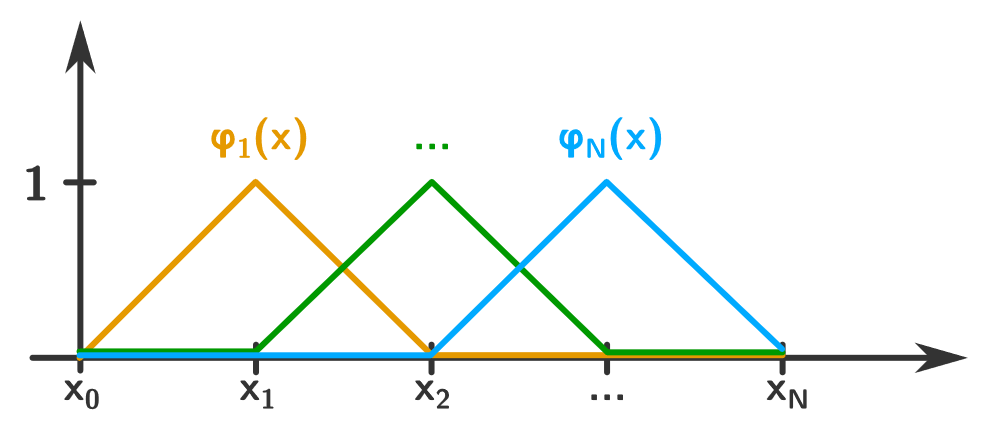
\includegraphics[width=3.54792in,height=1.55139in]{img/image17.png}Navážeme
% na předchozí příklad. Jako podprostor \(V_{h}\) pro Galerkinovu
% aproximaci zvolíme množinu lineárních lomených funkcí na intervalu (0,
% \emph{L}), konkrétně pro tento příklad s~nulovými Dirichletovými
% okrajovými podmínkami na obou stranách (\(u(0)\  = \ u(L)\  = \ 0\))
% bude vypadat takto:
% 
% Pokud bychom na jednom konci měli místo toho Neumannovu podmínku
% (\(- ku^{'}\left( L \right) = g\)), musíme na konec intervalu přidat
% funkci dosahující v~příslušném koncovém bodě hodnoty 1:
% 
% 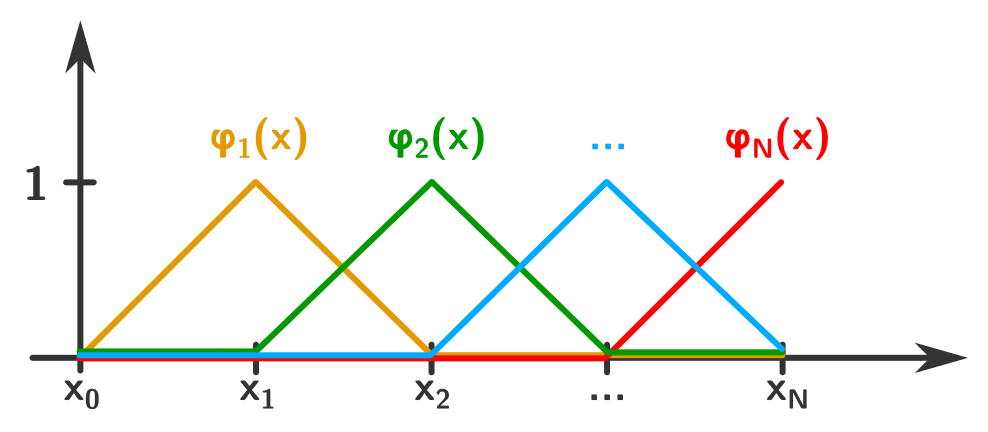
\includegraphics[width=3.54808in,height=1.55139in]{img/image19.png}
% 
% jinak bychom totiž nemohli lineární kombinací vytvořit funkci, která
% bude v~daném okrajovém bodě nenulová.
% 
% Interval (0, \emph{L}) rozdělíme pomocí bodů
% \(x_{0} = 0 < x_{1} < x_{2} < \ldots < x_{N} = L\) na podintervaly
% \(E_{j} := (x_{j - 1},x_{j})\) o délce \(h_{j} := x_{j} - x_{j - 1}\).
% Intervalům \(E_{j}\) říkáme \textbf{konečné prvky}. Místo integrace přes
% celý interval (0, \emph{L}), jak nám velí bodová formulace, budeme při
% využití MKP integrovat přes každý z těchto podintervalů zvlášť.
% 
% Dále zavedeme normu dělení: \(h := \max_{j = 1,\ldots,N}h_{j}\), tedy je
% to délka nejdelšího podintervalu vzniklého rozdělením intervalu (0,
% \emph{L}). Zatím pro zjednodušení uvažujme, že všechny podintervaly jsou
% stejně dlouhé a mají délku \(h\).
% 
% Nyní definujme prostor \(V_{h}\):
% 
% \(V_{h} :=´ \lbrack v_{h} \in C\left( \left\lbrack 0,\ L \right\rbrack \right):\ \forall j = 1,\ldots,N:\ v_{h}\)
% je lineární na
% \(E_{j},v_{h}\left( 0 \right) = v_{h}\left( L \right) = 0\)
% 
% Tedy:\(\ V_{h}\) je prostor lineárních funkcí \(v_{h}\), spojitých na
% (0, \emph{L}), pro které platí příslušné okrajové podmínky (pokud bychom
% v~bodě L měli Neumannovu podmínku, neplatí podmínka
% \(v_{h}\left( L \right) = 0\))
% 
% Jelikož funkce z prostoru \(V_{h}\) jsou spojité a splňují příslušné
% okrajové podmínky, je prostor \(V_{h}\) automaticky podprostorem \(V\) a
% navíc každou funkci \(v_{h}\) jednoznačně definují její hodnoty
% v~dělicích bodech \(\left\{ x_{j} \right\}_{j = 1}^{N}\).
% 
% 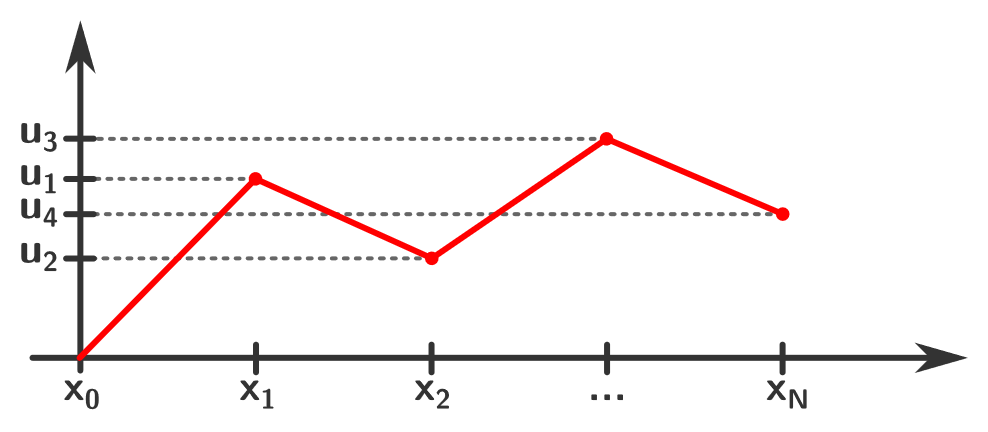
\includegraphics[width=3.54808in,height=1.55139in]{img/image21.png}Nějaká
% funkce \(u_{h}\) která patří do prostoru \(V_{h}\) může vypadat např.
% takto:
% 
% Pro funkční hodnoty v~bodech \(x_{i}\) platí:
% 
% \[u_{h}\left( x_{i} \right) = u_{i} = \sum_{j = 1}^{h}{u_{j}\varphi_{j}(x_{i})}\]
% 
% Podíváme-li se znovu na grafy bázových funkcí podprostoru \(V_{h}\),
% zjistíme, že platí:
% 
% \[\varphi_{j}\left( x_{i} \right) = \{\begin{matrix}
% \ 1\ \text{pokud}\ i = j \\
% \ 0\ \text{pokud}\ i \neq j \\
% \end{matrix} = \delta_{\text{ij}}\]
% 
% kde \(\delta_{\text{ij}}\) je Kroneckerovo delta -- funkce, která se
% rovná 1 pokud \(i = j\) a 0 ve všech ostatních případech. Díky tomu
% platí ona vlastnost funkcí z~prostoru \(V_{h}\), že jsou jednoznačně
% určeny hodnotami v~dělicích bodech, matematicky:
% 
% \[u_{h}\left( x_{i} \right) = u_{i}\varphi_{i}\left( x_{i} \right) = u_{i}\]
% 
% Dimenze podprostoru \(V_{h}\) je rovna \(N\), tedy počtu dělicích bodů.
% Z~dřívějška již víme, že volíme bázové funkce tak, že pro ně platí:
% \(\varphi_{i}\left( x_{j} \right): = \delta_{\text{ij}}\), každá bázová
% funkce je tedy nenulová právě v~jednom dělicím bodě (viz grafy dříve a
% na konci 1. přednášky).
% 
% Struktura matice \emph{A}:
% 
% Matici pro MKP \(A\) sestavíme z~prvků \(a_{\text{ij}}\) které vypočteme
% jako:
% 
% \[a_{\text{ij}} = \int_{0}^{L}{k(x)\varphi_{i}^{'}(x)}\varphi_{j}^{'}(x)dx\]
% 
% Vektor \(b\) sestává z~prvků \(b_{i}\), které určíme jako:
% 
% \[b_{i} = \int_{0}^{L}{f(x)\varphi_{i}'}dx + g\varphi_{i}(L)\]
% 
% Podíváme se podrobněji na výpočet \(a_{\text{ij}}\). Integrujeme
% postupně přes jednotlivé intervaly \(E_{e}\) (jednotlivé konečné prvky):
% 
% \[a_{\text{ij}} = \sum_{e = 1}^{N}{\int_{E_{e}}^{\ }{{{k(x)\varphi}_{i}^{'}(x)\varphi}_{j}^{'}(x)dx}}\]
% 
% 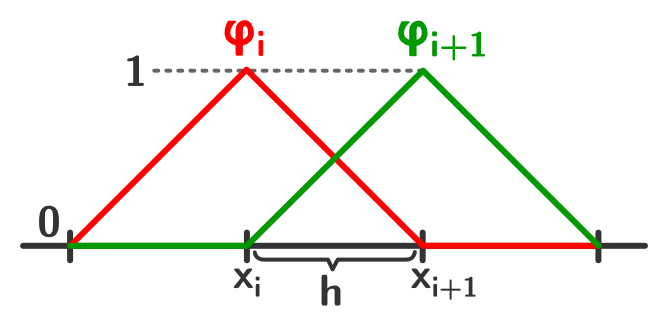
\includegraphics[width=2.89167in,height=1.38542in]{img/image23.png}integrál
% každé z~funkcí je nenulový pouze na určitém intervalu, protože bázové
% funkce jsou nenulové vždy pouze na a v~okolí jednoho dělicího bodu. Např
% pro \(a_{12}\) je integrál nenulový pouze na~intervalu
% (\(x_{1},\ x_{2}\)), všude jinde je buď \(\varphi_{i}\) nebo
% \(\varphi_{j}\) nulové, součin
% \({{k(x)\varphi}_{i}^{'}(x)\varphi}_{j}^{'}\) proto vychází 0.
% Prozkoumejme situaci obecně na intervalu (\(x_{i},\ x_{i + 1}\)):
% 
% \[a_{i,i + 1} = \int_{x_{i}}^{x_{i + 1}}{k\varphi_{i}'\varphi_{i + 1}'}\text{dx}\]
% 
% Derivace \(\varphi_{i}'\) je na daném intervalu záporná (\(\varphi_{i}\)
% klesá), velikost záleží na tom, jak prudce (z jaké hodnoty) klesá, např.
% v~tomto případě je derivace rovna \(\frac{- 1}{h}\).
% \(\varphi_{i + 1}'\) je kladné, v~tomto případě má velikost
% \(\frac{1}{h}\). Integrál je tedy roven:
% 
% \[a_{i,i + 1} = - \frac{1}{h^{2}}\int_{x_{i}}^{x_{i + 1}}k\text{dx}\]
% 
% 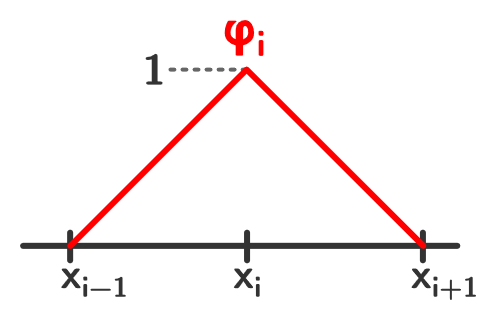
\includegraphics[width=2.09306in,height=1.35069in]{img/image25.png}Další
% nenulové prvky jsou \(a_{i,i}\), ty jsou rovny součtu dvou integrálů,
% protože součin \(\varphi_{i}\) sama se sebou je nenulový na dvou
% intervalech:
% 
% \[a_{i,i} = \int_{x_{i - 1}}^{x_{i}}{k\varphi_{i}'\varphi_{i}'}dx + \int_{x_{i}}^{x_{i + 1}}{k\varphi_{i}'\varphi_{i}'}\text{dx}\]
% 
% Na stoupající části je derivace rovna \(\frac{1}{h}\) a na klesající
% \(\frac{- 1}{h}\). Po dosazení:
% 
% \[a_{i,i} = \frac{1}{h^{2}}\int_{x_{i - 1}}^{x_{i}}kdx + \frac{1}{h^{2}}\int_{x_{i}}^{x_{i + 1}}k\text{dx}\]
% 
% pro jednoduchost uvažujme, že funkce \(k\)~je po částech konstantní a na
% intervalu \(E_{i}\) je rovna konstantě \(k_{i}\). Matice \(A\) má tři
% nenulové diagonály:
% 
% \[\begin{bmatrix}
% a_{i,i} & a_{i,i + 1} & 0 & 0 & \cdots & 0 \\
% a_{i - 1,i} & a_{i,i} & a_{i,i + 1} & 0 & \ddots & \vdots \\
% 0 & a_{i - 1,i} & \cdots & \cdots & 0 & 0 \\
% 0 & 0 & \cdots & \cdots & a_{i,i + 1} & 0 \\
%  \vdots & \ddots & 0 & a_{i - 1,i} & a_{i,i} & a_{i,i + 1} \\
% 0 & \cdots & 0 & 0 & a_{i - 1,i} & a_{i,i} \\
% \end{bmatrix}\]
% 
% a my již víme, jak jednotlivé nenulové prvky spočítat. Při po částech
% konstantním \(k\)~platí:
% 
% \[a_{i,i} = \frac{1}{h}\left( k_{i} + k_{i + 1} \right)\]
% 
% \[a_{i - 1,i} = a_{i,i + 1} = - \frac{1}{h}k_{i}\]
% 
% např pro \(k_{i} = k_{i + 1} = k = 1\) vypadá matice následovně:
% 
% \[\frac{1}{h}\begin{bmatrix}
% 2 & - 1 & 0 & 0 & \cdots & 0 \\
%  - 1 & 2 & - 1 & 0 & \ddots & \vdots \\
% 0 & - 1 & \cdots & \cdots & 0 & 0 \\
% 0 & 0 & \cdots & \cdots & - 1 & 0 \\
%  \vdots & \ddots & 0 & - 1 & 2 & - 1 \\
% 0 & \cdots & 0 & 0 & - 1 & 2 \\
% \end{bmatrix}\]
% 
% Podobným způsobem lze odvodit i podobu jednotlivých členů vektoru \(b\),
% tím se teď nebudeme zabývat.
% 
% Jak jsme již zmínili na konci minulé hodiny, výhodou matice \(A\) je to,
% že je \textbf{řídká}, tedy obsahuje jen málo nenulových prvků. Proto se
% s~ní dobře pracuje, zejména u úloh, které mají hodně stupňů volnosti
% (jejich matice \(A\) bude mít hodně řádků a sloupců). V~praxi je žádoucí
% co největší počet stupňů volnosti, protože čím je jich více, tím
% přesněji lze aproximovat řešení. I velmi velkou matici \(A\) lze uložit
% do poměrně malého počítačového souboru, protože stačí zaznamenat hodnoty
% na nenulových pozicích.
% 
% Matice \(A\) je řídká proto, že jednotlivé bázové funkce prostoru
% \(V_{h}\) jsou na většině intervalu nulové, součiny jejich derivací
% s~čímkoliv dalším jsou proto taky nulové. Nenulové oblasti bázové funkce
% se říká \textbf{nosič}, bázové funkce mají nosič malý a na většině
% intervalu je \textbf{disjunktní}, tedy nemá nenulový průnik s~jinými
% bázovými funkcemi.
% 
% \hypertarget{poissonova-rovnice-ve-2d}{%
% \section{Poissonova rovnice ve 2D}\label{poissonova-rovnice-ve-2d}}
% 
% Rovnice vedení tepla ve 2D:
% 
% 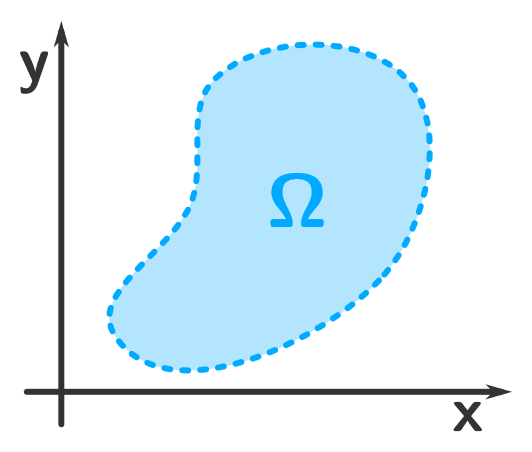
\includegraphics[width=1.51042in,height=1.28264in]{img/image27.png}Začneme
% definováním oblasti (množiny), na které budeme počítat. Tu označíme $\Omega$ a
% musí mít následující vlastnosti:
% 
% \begin{itemize}
% \item
%   Otevřená -- nepatří do ní její hranice
% \item
%   Jednoduše souvislá -- celá oblast sestává pouze z~jednoho „kusu``,
%   není rozdělená na více nepropojených oblastí, ani neobsahuje „díry``.
% \end{itemize}
% 
% Nyní zapíšeme rovnici vedení tepla pro dvě dimenze:
% 
% \[\text{div}\ ( - \left( k\left( \overrightarrow{x} \right) \bullet \nabla u\left( \overrightarrow{x} \right) \right)) = f(\overrightarrow{x})\]
% 
% vidíme že ve 2D je rovnice složitější, vyskytují se zde následující
% operátory:
% 
% \begin{itemize}
% \item
%   \(\nabla\) \emph{= gradient -- vektor, který má následující
%   podobu:}\(\ \nabla\  = \left( \frac{\partial}{\partial x},\ \ \frac{\partial}{\partial y},\ \ \frac{\partial}{\partial z} \right)\)
% \item
%   \emph{div = divergence -- představuje skalární součin funkce
%   s~gradientem:} \(\text{div}\left( f(x) \right) = \nabla \bullet f(x)\)
% \end{itemize}
